\documentclass{article}
\usepackage[backend=biber, style=numeric, citestyle=numeric]{biblatex}
\addbibresource{ref.bib}
\usepackage{graphicx}
\usepackage{amsmath, bm, amssymb}
\usepackage{titlesec}
\usepackage{geometry}
\usepackage{fancyhdr}
\usepackage{xcolor}
\usepackage{algorithm}
\usepackage{algpseudocode}
\geometry{left=1in, right=1in, top=1in, bottom=1in}

\definecolor{titlecolor}{RGB}{0, 0, 128}

\titleformat{\section}[block]{\normalfont\Large\bfseries\color{titlecolor}}{\thesection}{1em}{}
\titleformat{\subsection}[block]{\normalfont\large\bfseries\color{titlecolor}}{\thesubsection}{1em}{}

\pagestyle{fancy}
\fancyhf{}
\lhead{\scriptsize EEC 289A Assignment 1 Report}
\rhead{}
\cfoot{\thepage}

\begin{document}

\noindent
\textbf{\large EEC 289A Assignment 1 Report} \\
\textbf{\small Chenye Yang, Hanchu Zhou, Haodong Liang, Yibo Ma}


\vspace{2mm}

\section{Introduction}

In this project, we aim to do K-mean clustering on the patches from MNIST dataset. After the clustering, we observe the results, and try to answer the following interesting questions:

\begin{itemize}
    \item The number of clusters required to cover the whole patch space
    \item The interpretable meaning of the clusters
    \item The connection between the digit and the patches
    \item ???
\end{itemize}

\vspace{2mm}

\section{Methodology}

Firstly, we load the MNIST data and crop the 28 $\times$ 28 hand-written digits to 5$\times$ 5 digits with a moving filter. Therefore, for each hand-write digit, we will get $(28 -5 +1) \times (28 - 5 + 1)$ patches, and then we get rid of all the blank patches. After we get all the useful patches, there are mainly two parts in this project:

\begin{itemize}
    \item K-mean clustering to generate the centroids and corresponding subsets
    \item Reconstruction with the centroids to test the performance
\end{itemize}


\vspace{2mm}

\subsection{K-mean clustering}

We define that:

\begin{itemize}
    \item $K:$ Number of the clustering 
    \item $C:$ Centroids of the clustering
    \item $P:$ The 5 $\times$ 5 patch
    \item $\vec{x}: $ The values of the 25 pixels, $\vec{x} \in R^{25 \times 1}$
\end{itemize}


\vspace{2mm}

The overall algorithm is as shown as below, and we test with K = 100, 200, ..., 900, 1000, 2000, 3000, ..., 10000, and we show the experiment results in section \mathbf{3}.

\begin{algorithm}
\caption{Enhanced K-means Clustering for $5 \times 5$ Patches}
\begin{algorithmic}[1]
\Procedure{KMeansPatches}{$Patches, K$}
    \State $X \gets \text{Reshape each patch } P \text{ in } Patches \text{ to } R^{25}$
    \State Initialize $C$ with K-means++ to choose $K$ centroids from $X$
    \State $C_{\text{old}} \gets \text{Copy of } C$
    \Repeat
        \State Compute distances from each vector $X_i$ in $X$ to each centroid in $C$
        \State Assign each vector $X_i$ to the closest centroid
        \For{$j \gets 1$ \text{to} $K$}
            \If{$\text{Count}(X_i \text{ assigned to } C_j) = 0$}
                \State Randomly reinitialize centroid $C_j$ from $X$
            \Else
                \State Update centroid $C_j$ by calculating the mean of all vectors assigned to $C_j$
            \EndIf
        \EndFor
        \State $C_{\text{new}} \gets \text{Copy of } C$
        \State $C_{\text{move}} \gets \text{norm}(C_{\text{new}} - C_{\text{old}})$
        \State $C_{\text{old}} \gets C_{\text{new}}$
    \Until{$C_{\text{move}} < \text{tolerance}$}
    \State \Return Updated centroids and cluster labels
\EndProcedure
\end{algorithmic}
\end{algorithm}



\vspace{2mm}

\subsection{Reconstruction}

As for the reconstruction, it is used to test the performance. The algorithm is as shown in the algorithm 2.

\vspace{2mm}

Some notations in this algorithm:

\begin{itemize}
    \item $POS$: The position indice of a specific patch
    \item $D$: The ground truth of the hand-written digit 
    \item $\hat{D}$: The reconstructed result of $D$ according to the K-mean clustering results
\end{itemize}


\begin{algorithm}
\caption{Testing K-means Clustering on Handwritten Digit Images}
\begin{algorithmic}[1]
\Procedure{ReconstructDigit}{$D, K, Model$}
    \State $P \gets \text{empty list to store patches}$
    \State $Pos \gets \text{empty list to store position indices}$
    \For{$i \gets 1 \text{ to } 24$} \Comment{28 - 5 + 1 = 24}
        \For{$j \gets 1 \text{ to } 24$}
            \State $patch \gets D[i:i+5, j:j+5]$
            \If{$\text{not all zeros in } patch$}
                \State $P.\text{append}(patch.flatten())$
                \State $Pos.\text{append}((i, j))$
            \EndIf
        \EndFor
    \EndFor
    \State $X \gets \text{stack of patches in } P$
    \State $Labels \gets Model.\text{predict}(X)$ \Comment{Assign clusters to patches}
    \State $\hat{D} \gets \text{zero matrix of the same size as } D$ \Comment{Initialize reconstructed digit with zeros}
    \For{$k \gets 0 \text{ to } \text{len}(P)-1$}
        \State $pos \gets Pos[k]$
        \State $cluster \gets Labels[k]$
        \State $centroid \gets Model.cluster\_centers_[cluster].reshape(5, 5)$
        \State $\hat{D}[pos[0]:pos[0]+5, pos[1]:pos[1]+5] \gets centroid$
    \EndFor
    \State \Return $\hat{D}$
\EndProcedure
\end{algorithmic}
\end{algorithm}


\clearpage

\section{Experiment Results}

% \textbf{We don't do normalization in our experiment, which means that the pixel value is either 0 or 255.}

\quad

For the experiment results, it is divded into three parts:

\begin{itemize}
    \item Number of clusters required to cover the whole pacth space
    \item Interpretable meaning of the clusters
    \item Connection between the digit and the patches
\end{itemize}

\subsection{Selection of $K$}

With different values of $K$, we can get different clustering results, and we here show the results of the clustering of different $K$, patches combined with the corresponding centroids.

\begin{itemize}
    \item $K = 100$
    \begin{figure}[htbp!]
        \centering
        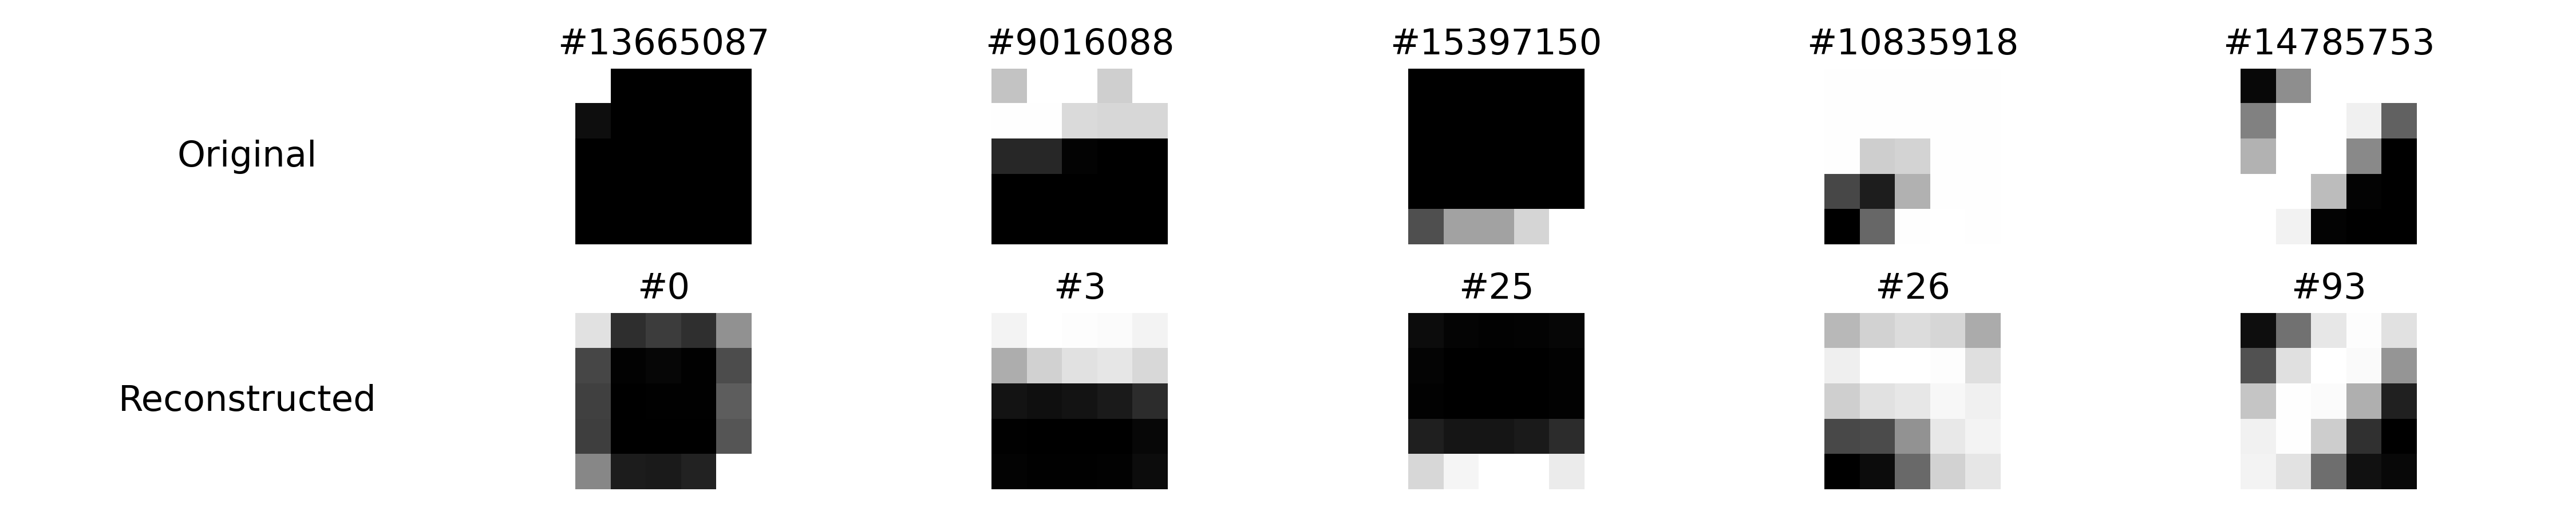
\includegraphics[width = 0.9 \textwidth]{K-means/Result/Patches/100-clusters-reconstruction.png}
        \caption{The patch and corresponding centroid when $K = 100$}
        \label{fig:enter-label}
    \end{figure}

        \item $K = 200$
    \begin{figure}[htbp!]
        \centering
        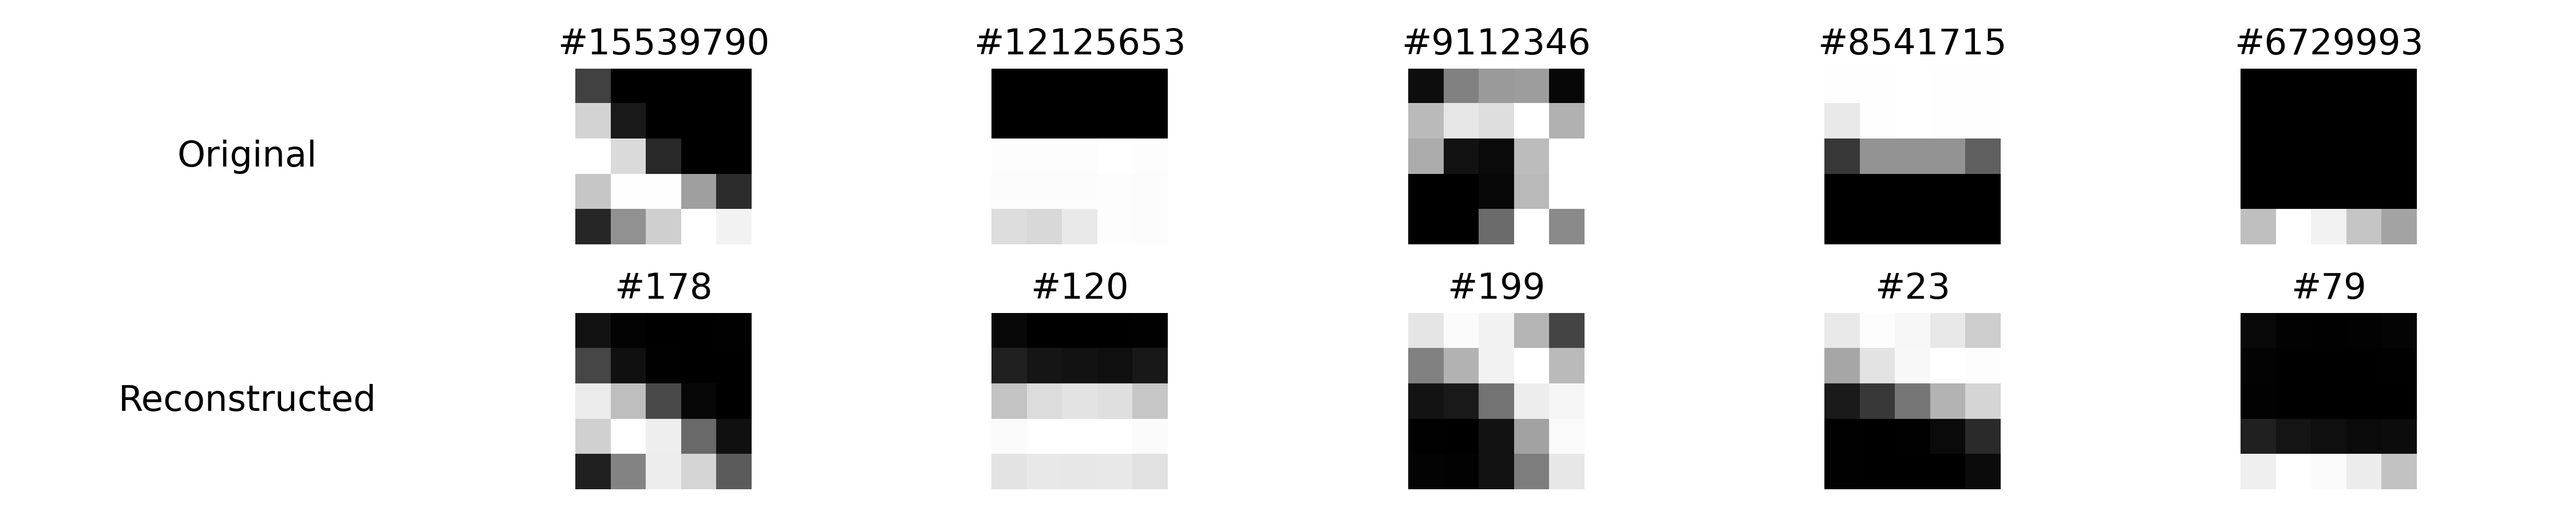
\includegraphics[width = 0.9 \textwidth]{K-means/Result/Patches/200-clusters-reconstruction.png}
        \caption{The patch and corresponding centroid when $K = 200$}
        \label{fig:enter-label}
    \end{figure}

        \item $K = 400$
    \begin{figure}[htbp!]
        \centering
        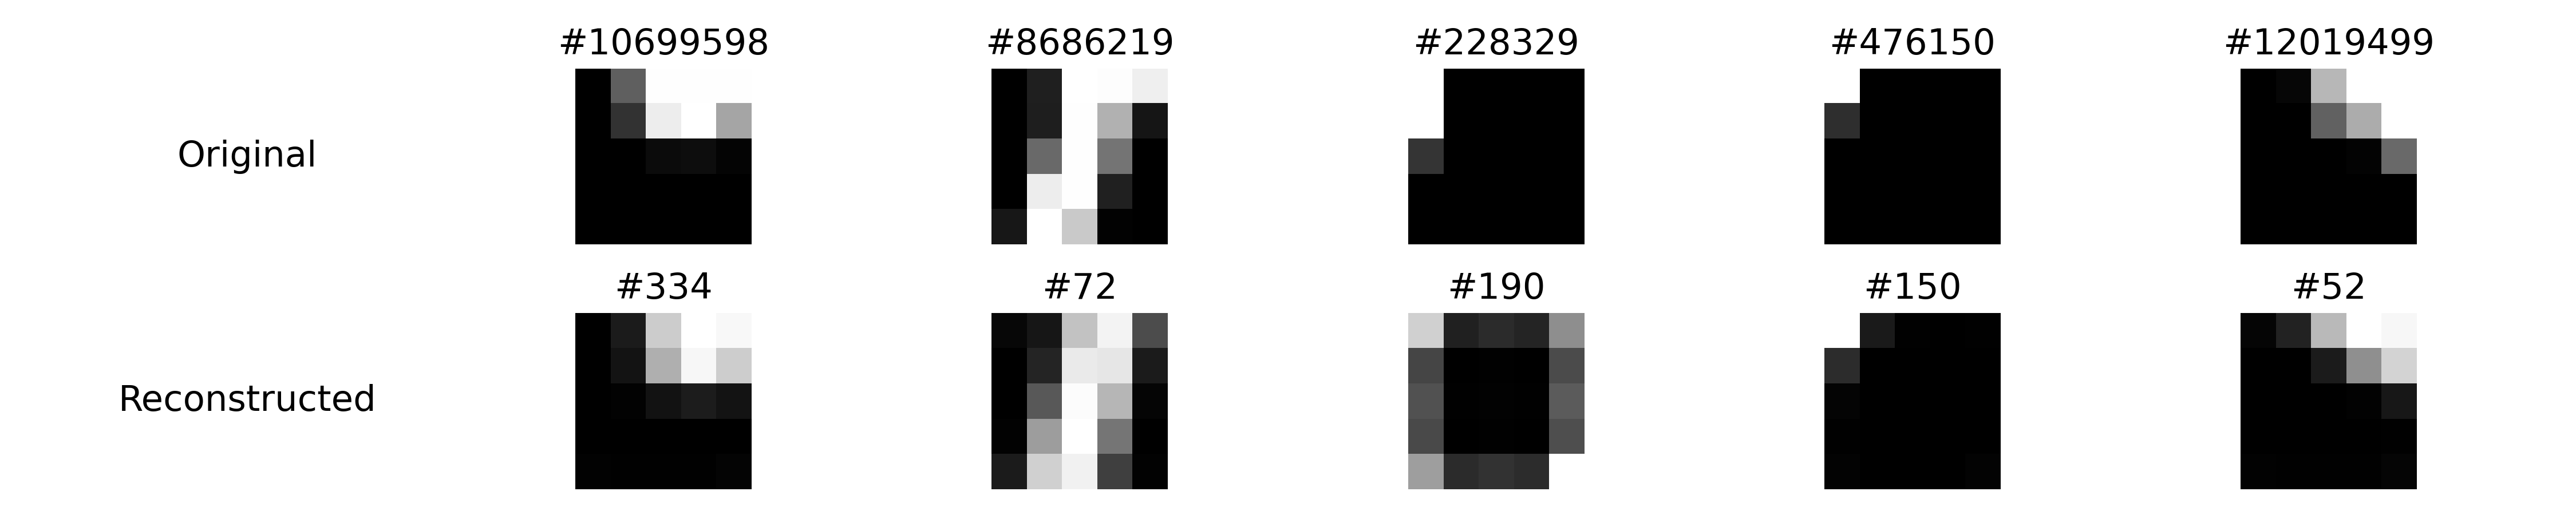
\includegraphics[width = 0.9 \textwidth]{K-means/Result/Patches/400-clusters-reconstruction.png}
        \caption{The patch and corresponding centroid when $K = 400$}
        \label{fig:enter-label}
    \end{figure}
    \clearpage

        \item $K = 1000$
    \begin{figure}[htbp!]
        \centering
        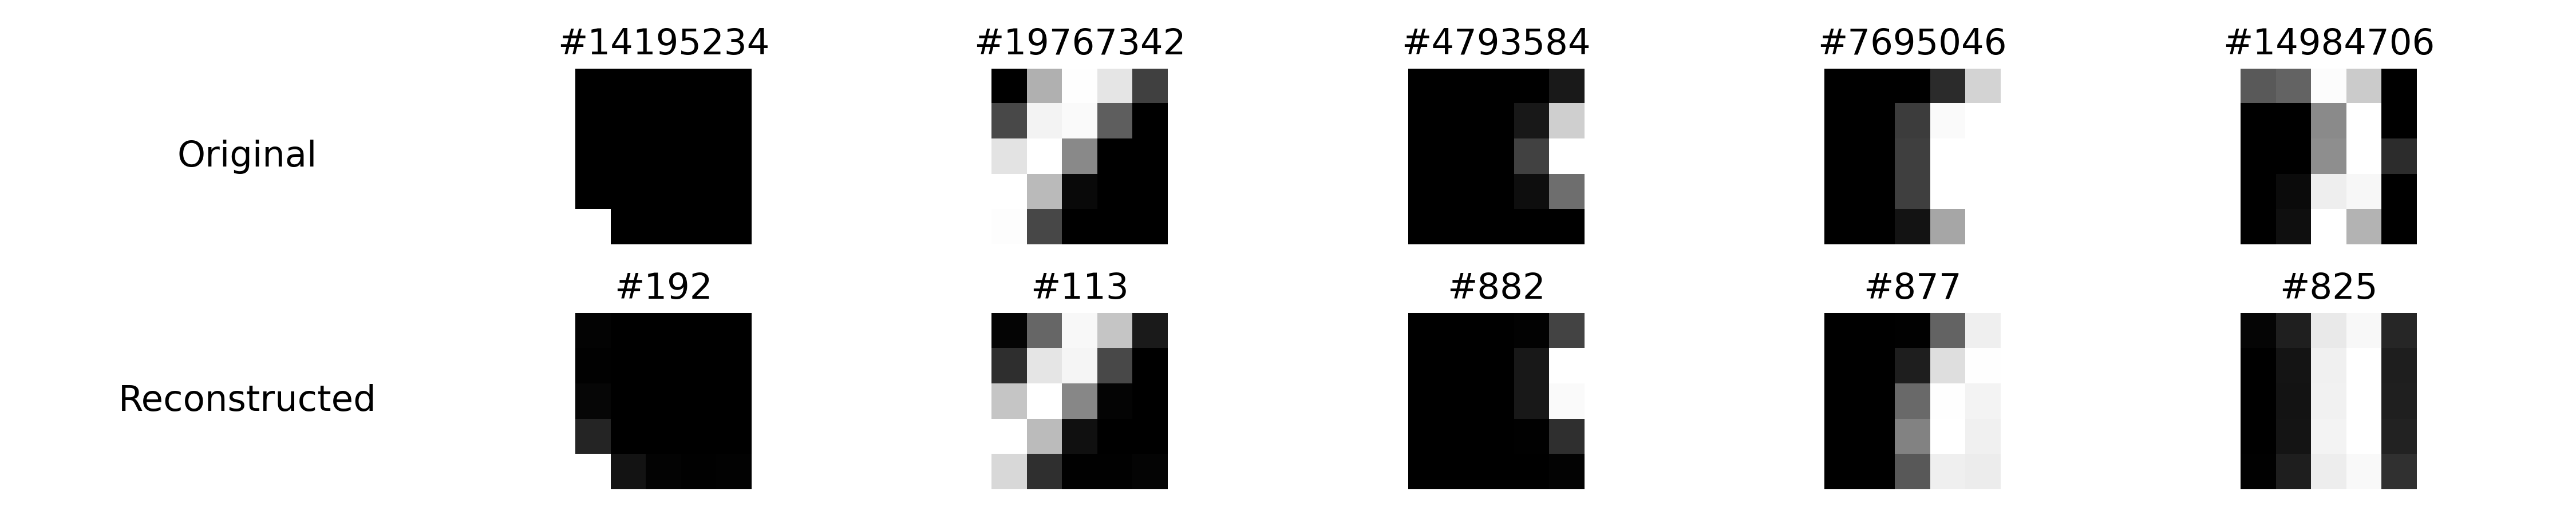
\includegraphics[width = 0.9 \textwidth]{K-means/Result/Patches/1000-clusters-reconstruction.png}
        \caption{The patch and corresponding centroid when $K = 1000$}
        \label{fig:enter-label}
    \end{figure}

            \item $K = 5000$
    \begin{figure}[htbp!]
        \centering
        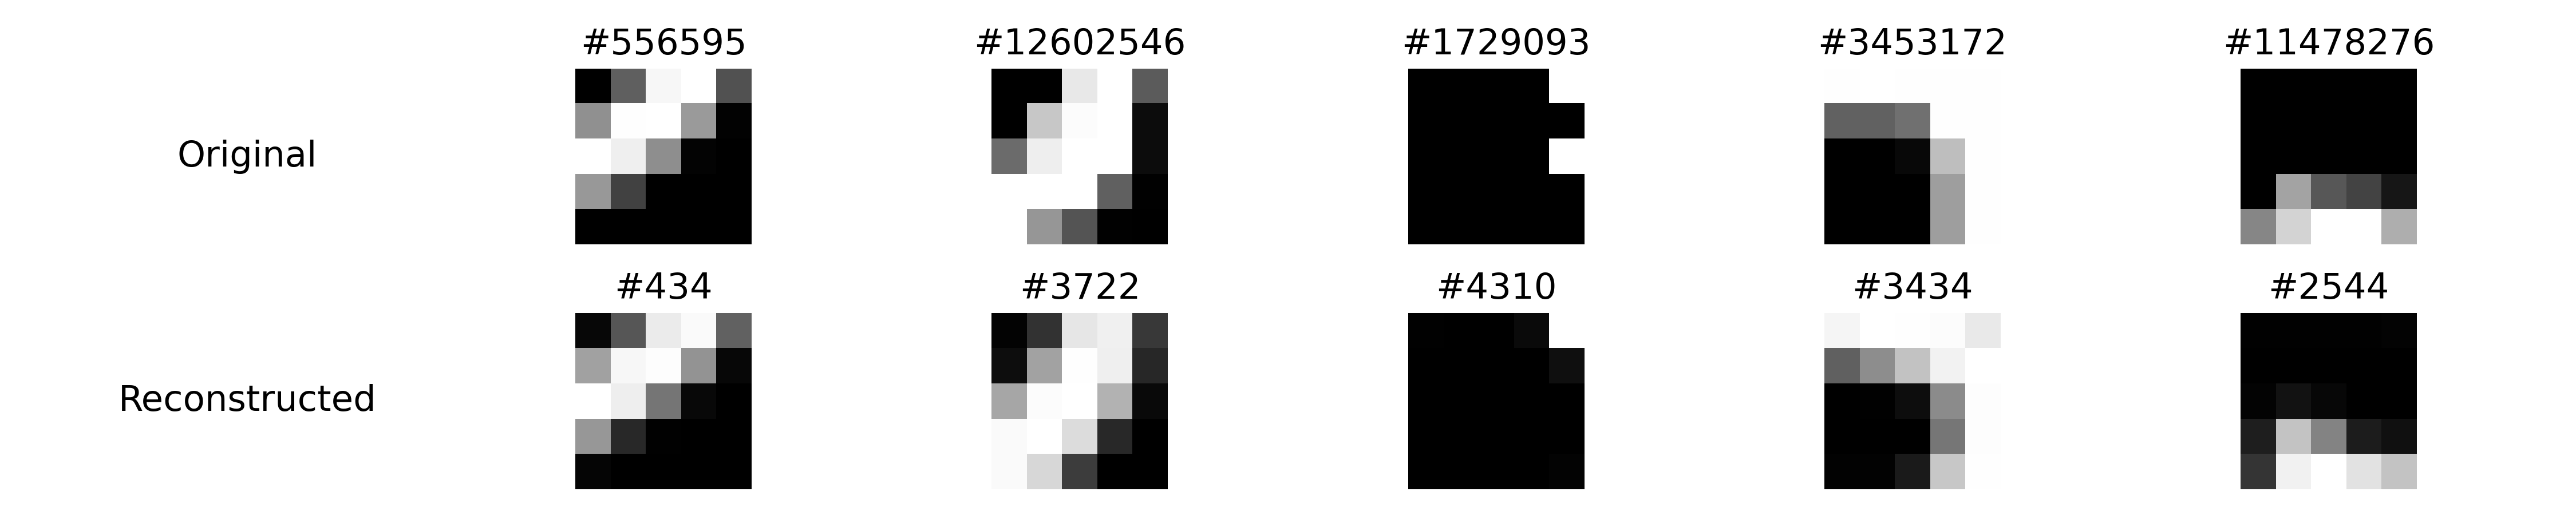
\includegraphics[width = 0.9 \textwidth]{K-means/Result/Patches/5000-clusters-reconstruction.png}
        \caption{The patch and corresponding centroid when $K = 5000$}
        \label{fig:enter-label}
    \end{figure}

        \item $K = 10000$
    \begin{figure}[htbp!]
        \centering
        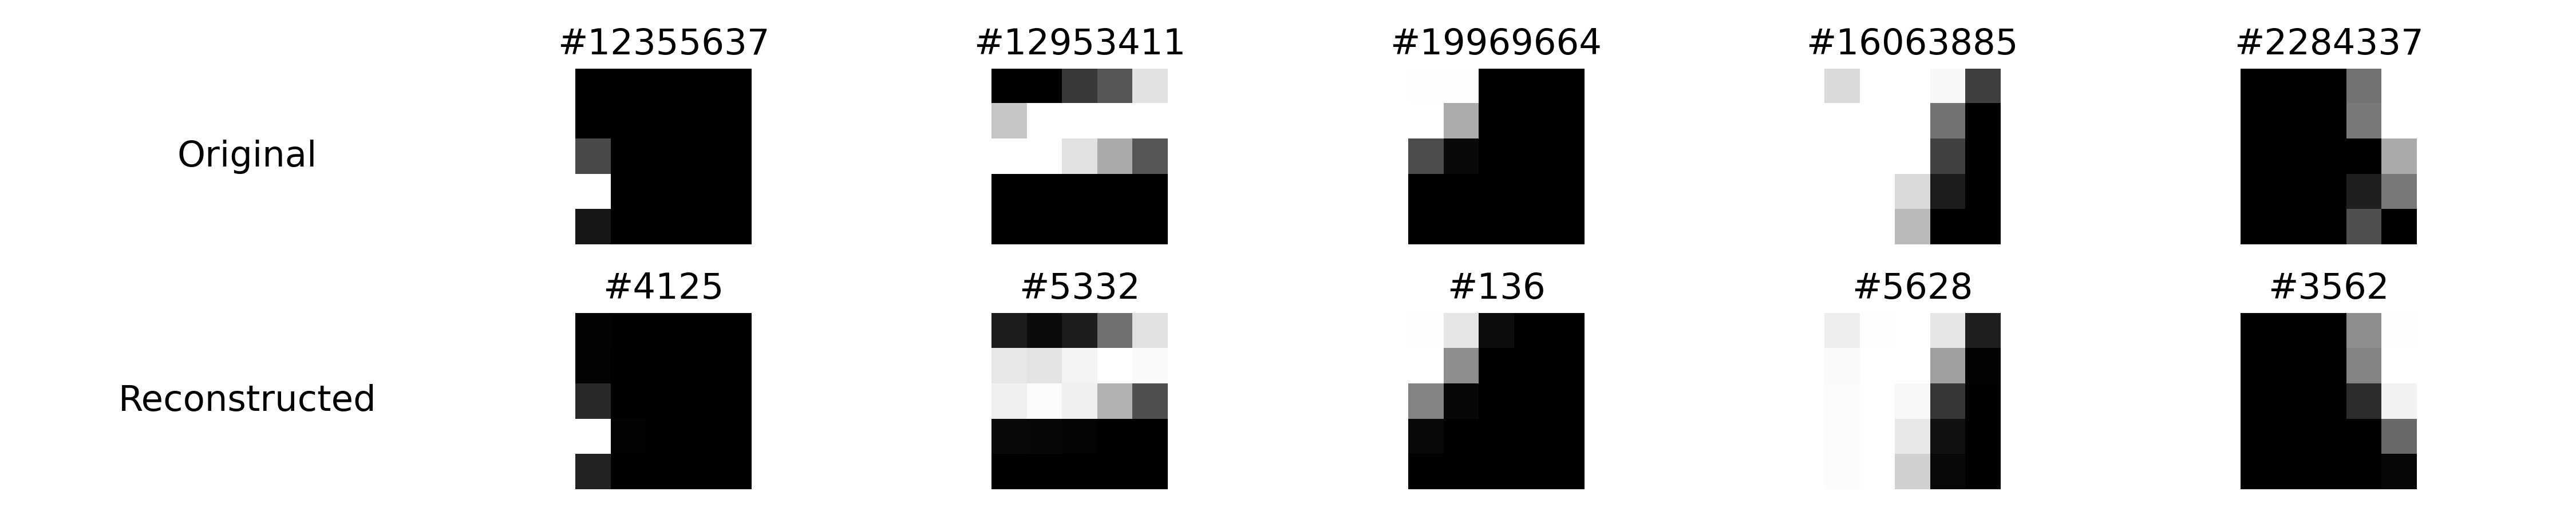
\includegraphics[width = 0.9 \textwidth]{K-means/Result/Patches/10000-clusters-reconstruction.png}
        \caption{The patch and corresponding centroid when $K = 10000$}
        \label{fig:enter-label}
    \end{figure}
    
\end{itemize}

With the results above, we can observe that:

\begin{itemize}
    \item As K increases, the original figure and reconstructed figure tends to be more similar.
    \item When K=10000, the reconstructed figure can almost recover all details of the original patches.
\end{itemize}


\subsection{Meaning of $C$}

In addition to the clustering performance, we also want to understand the meaning of the clusters or centroids. Here we show the results of the centroids given different $K$:


\begin{itemize}
\begin{figure}[htbp!]
\item $K = 100, 200$
    \centering
    % First row
    \begin{minipage}{0.4\textwidth}
        \centering
        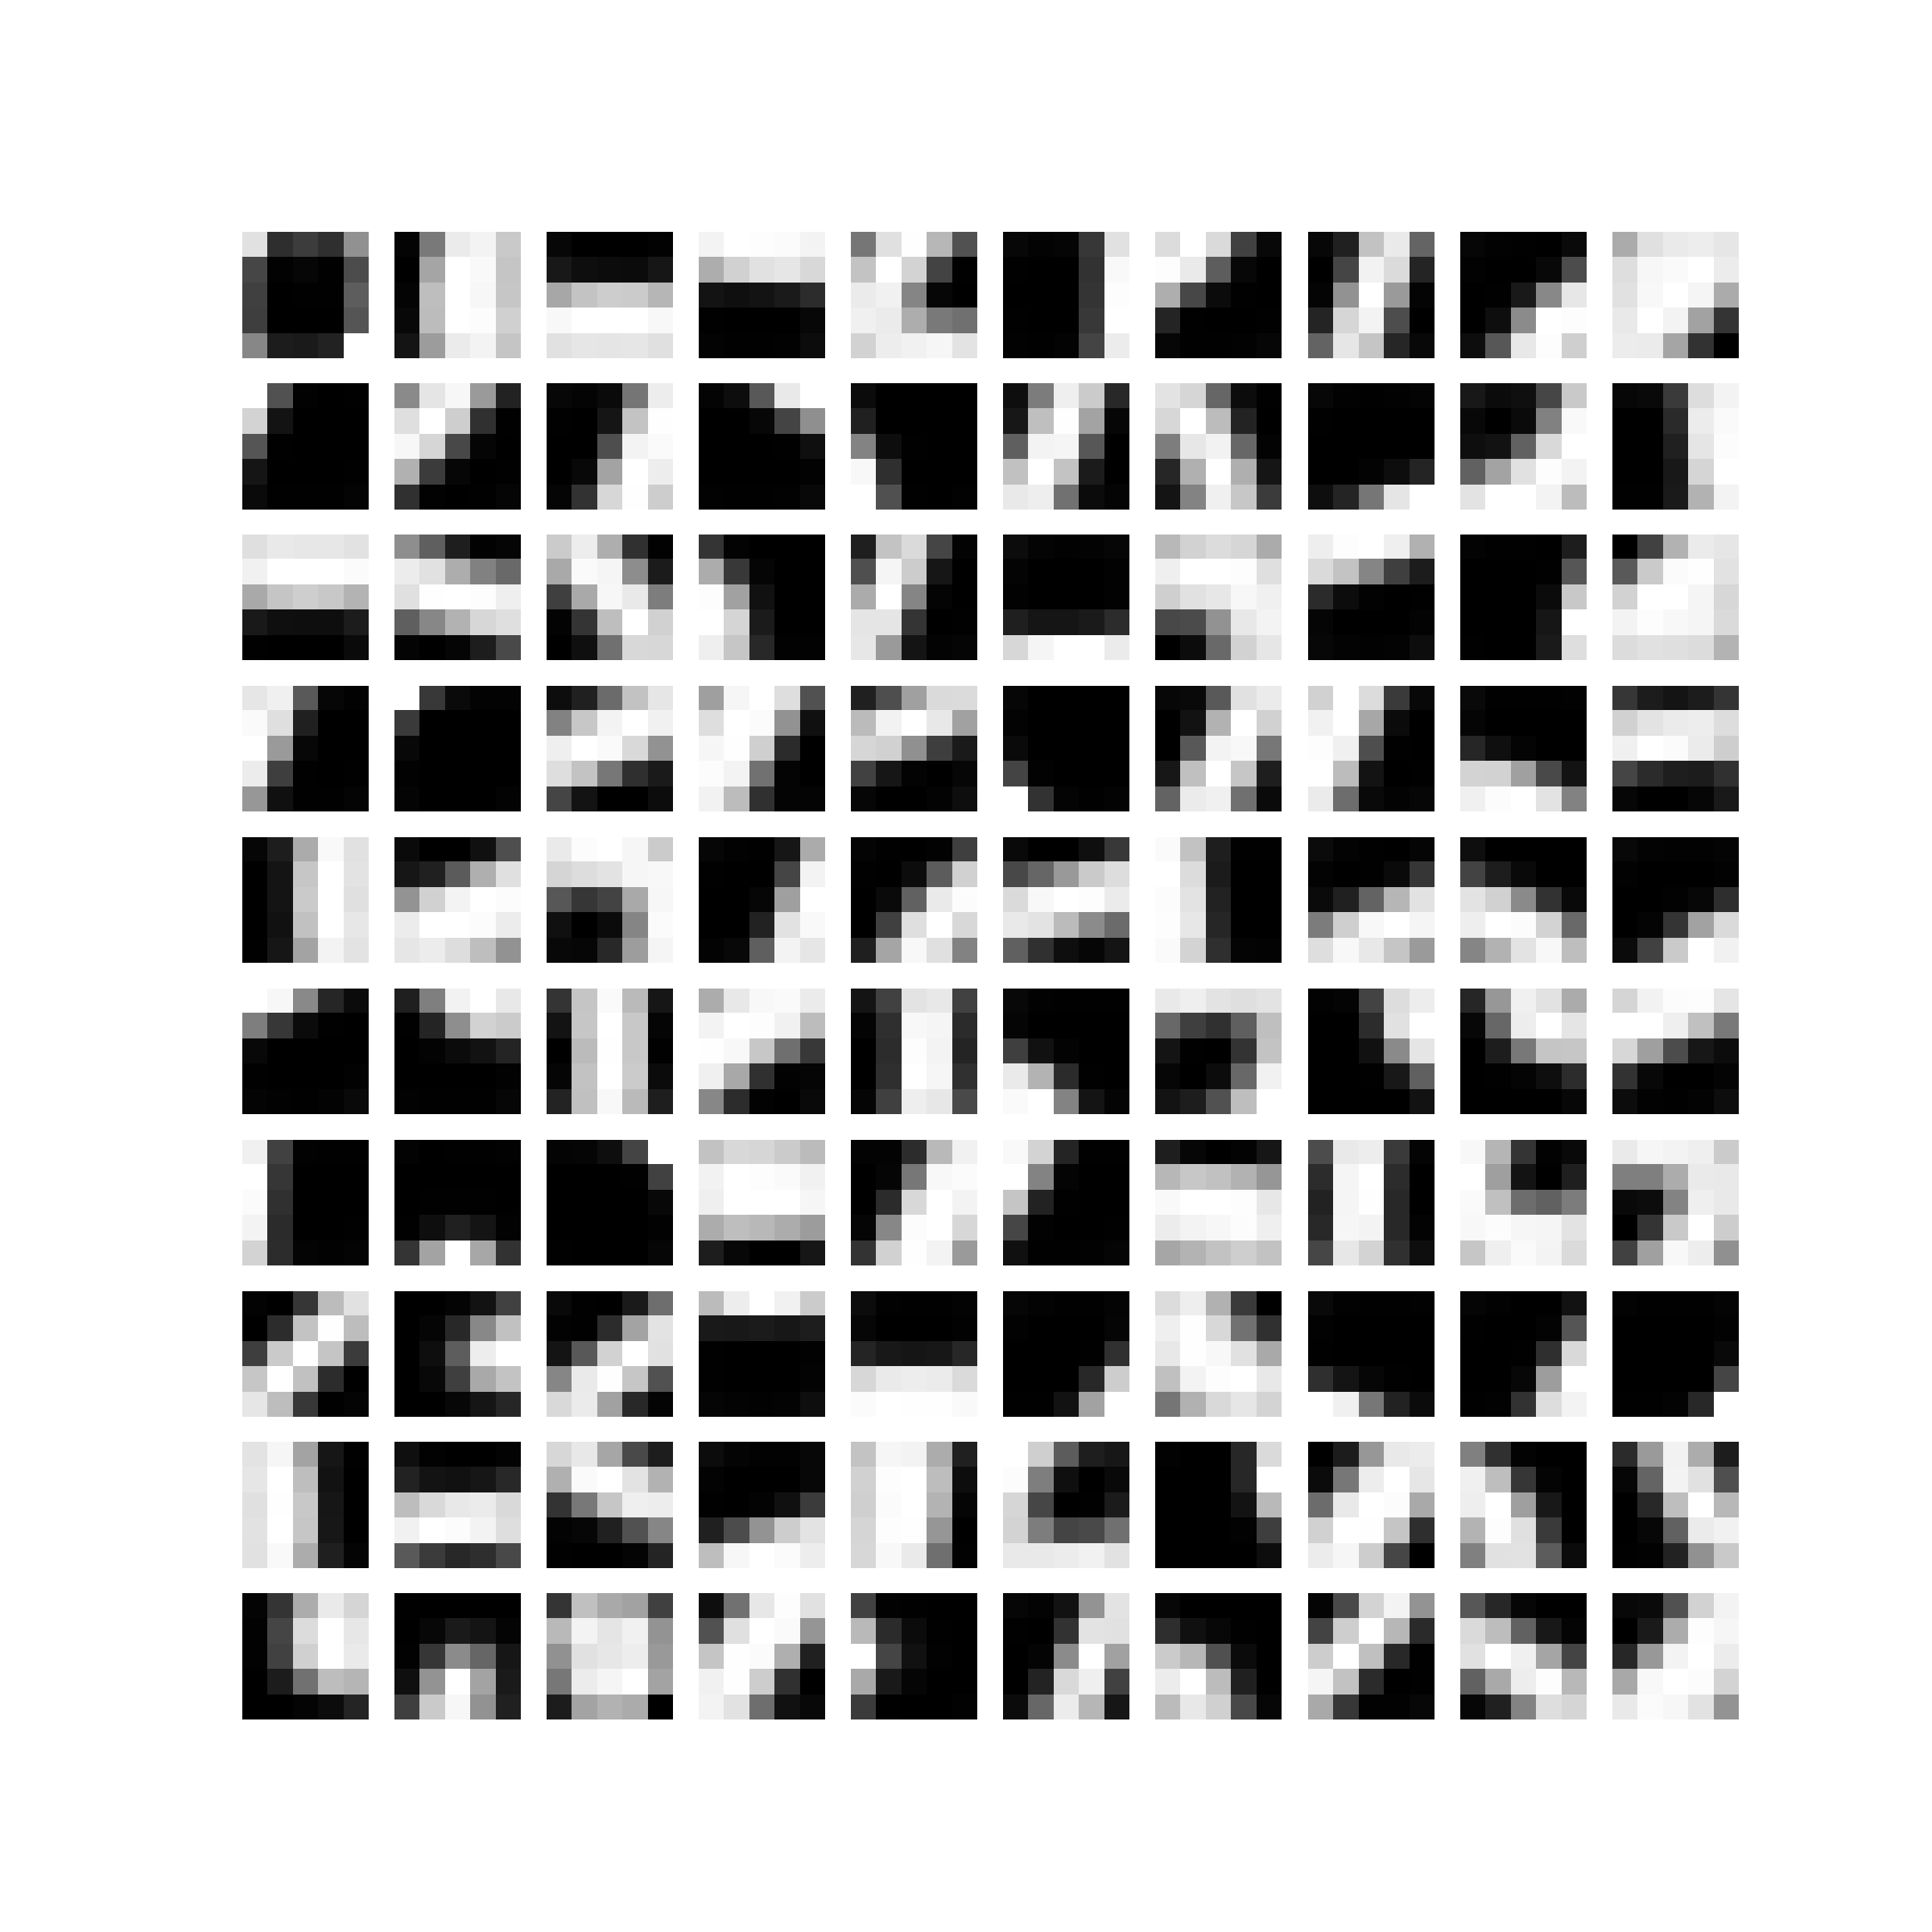
\includegraphics[width=\textwidth]{K-means/Result/Centroids/100-clusters-centroids.png}
        \caption{$K = 100$}
        \label{fig:100-centroids}
    \end{minipage}%
    \begin{minipage}{0.4\textwidth}
        \centering
        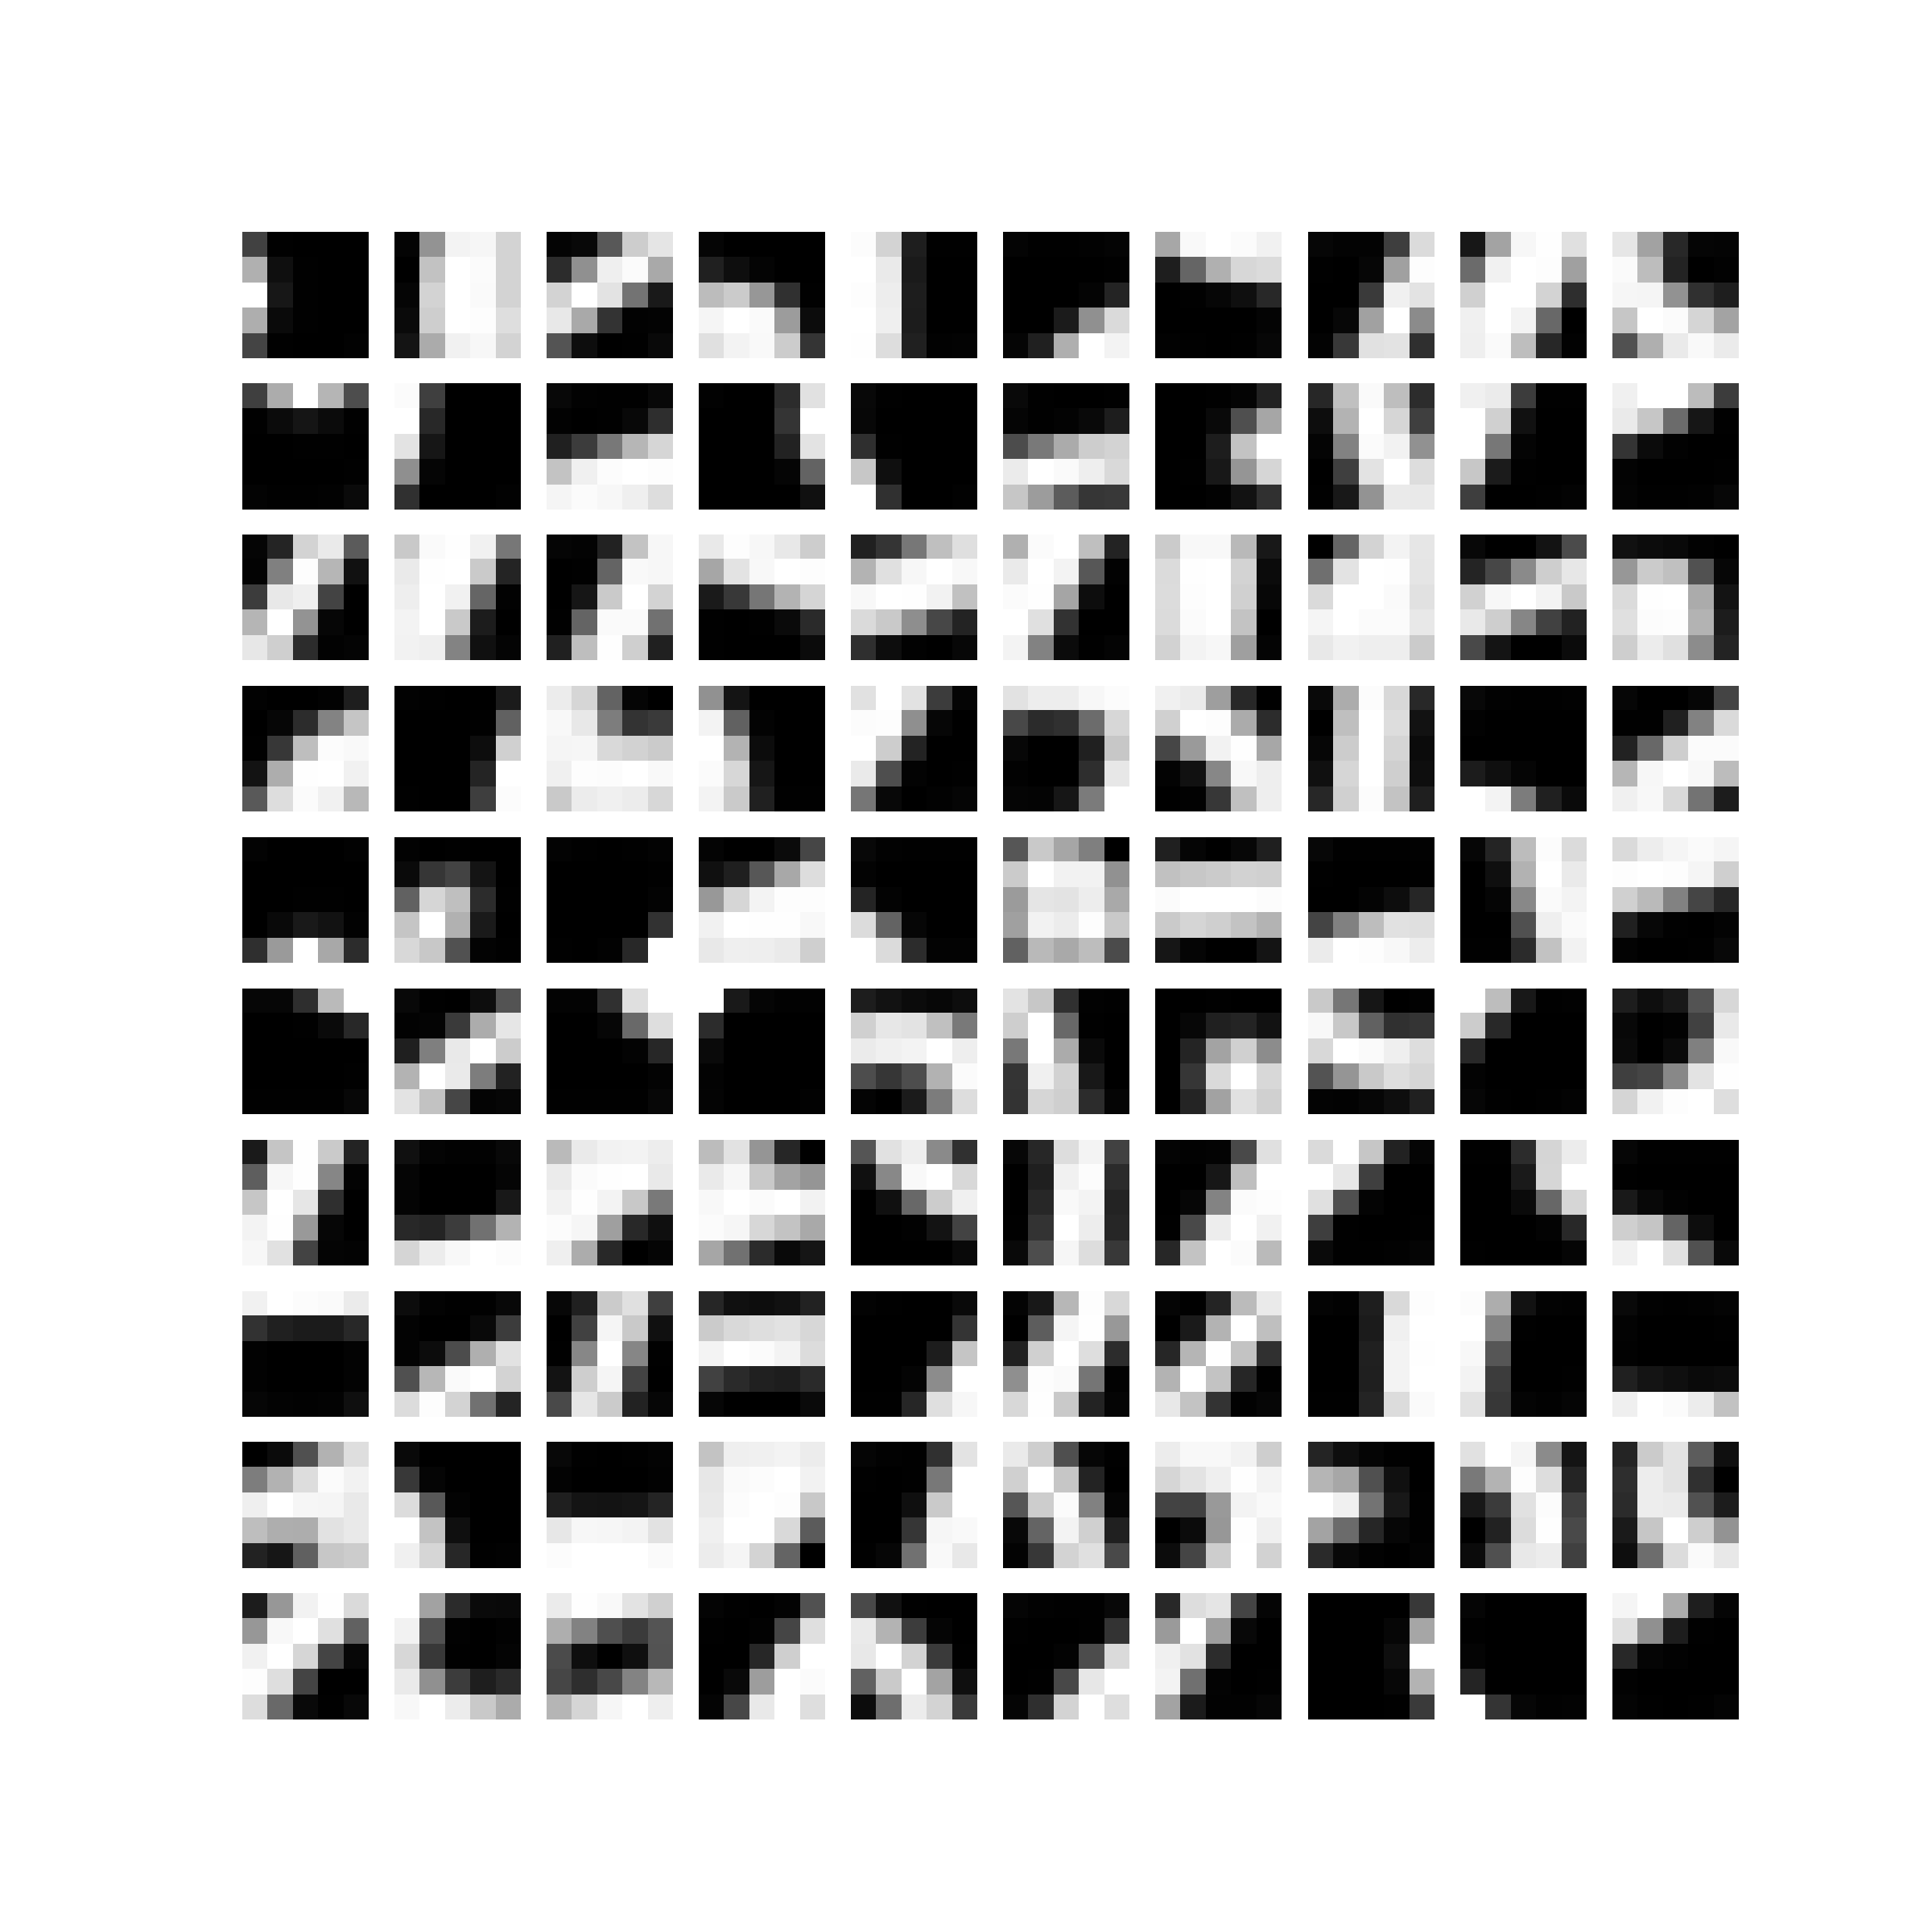
\includegraphics[width=\textwidth]{K-means/Result/Centroids/200-clusters-centroids.png}
        \caption{$K = 200$}
        \label{fig:200-centroids}
    \end{minipage}
\item $K = 400, 1000$    
    % Second row
    \begin{minipage}{0.4\textwidth}
        \centering
        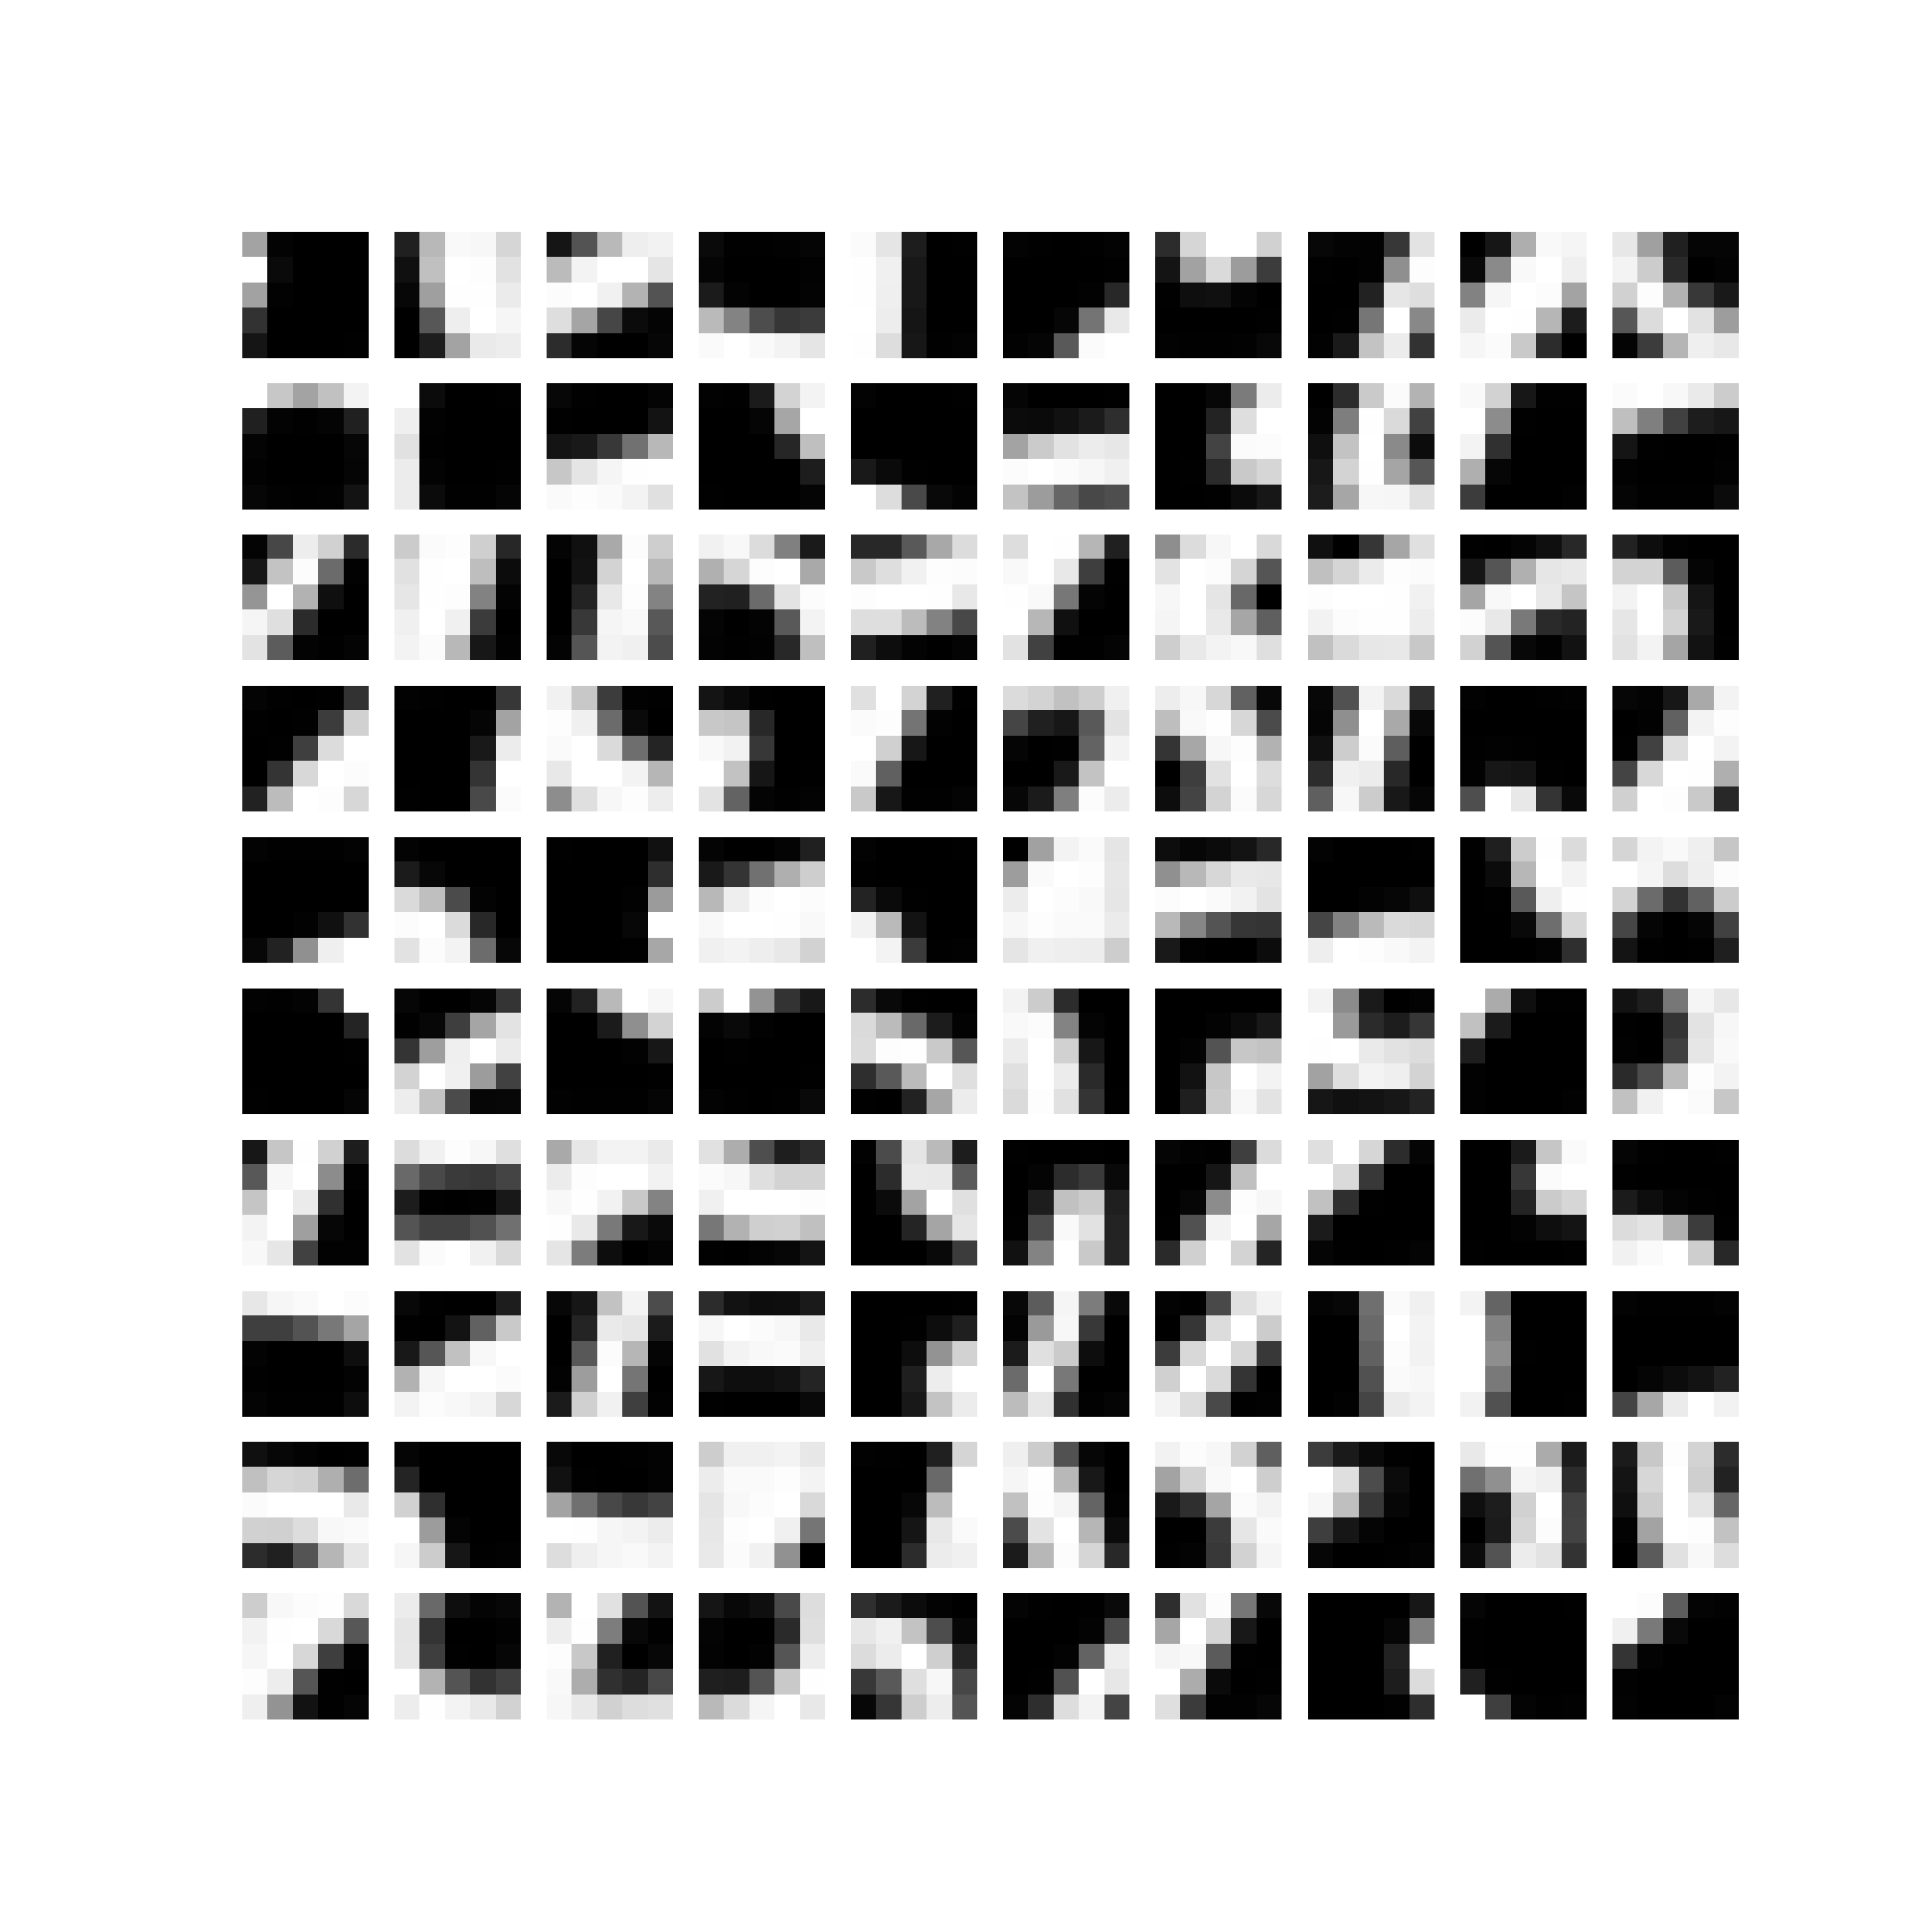
\includegraphics[width=\textwidth]{K-means/Result/Centroids/400-clusters-centroids.png}
        \caption{$K = 400$}
        \label{fig:400-centroids}
    \end{minipage}%
    \begin{minipage}{0.4\textwidth}
        \centering
        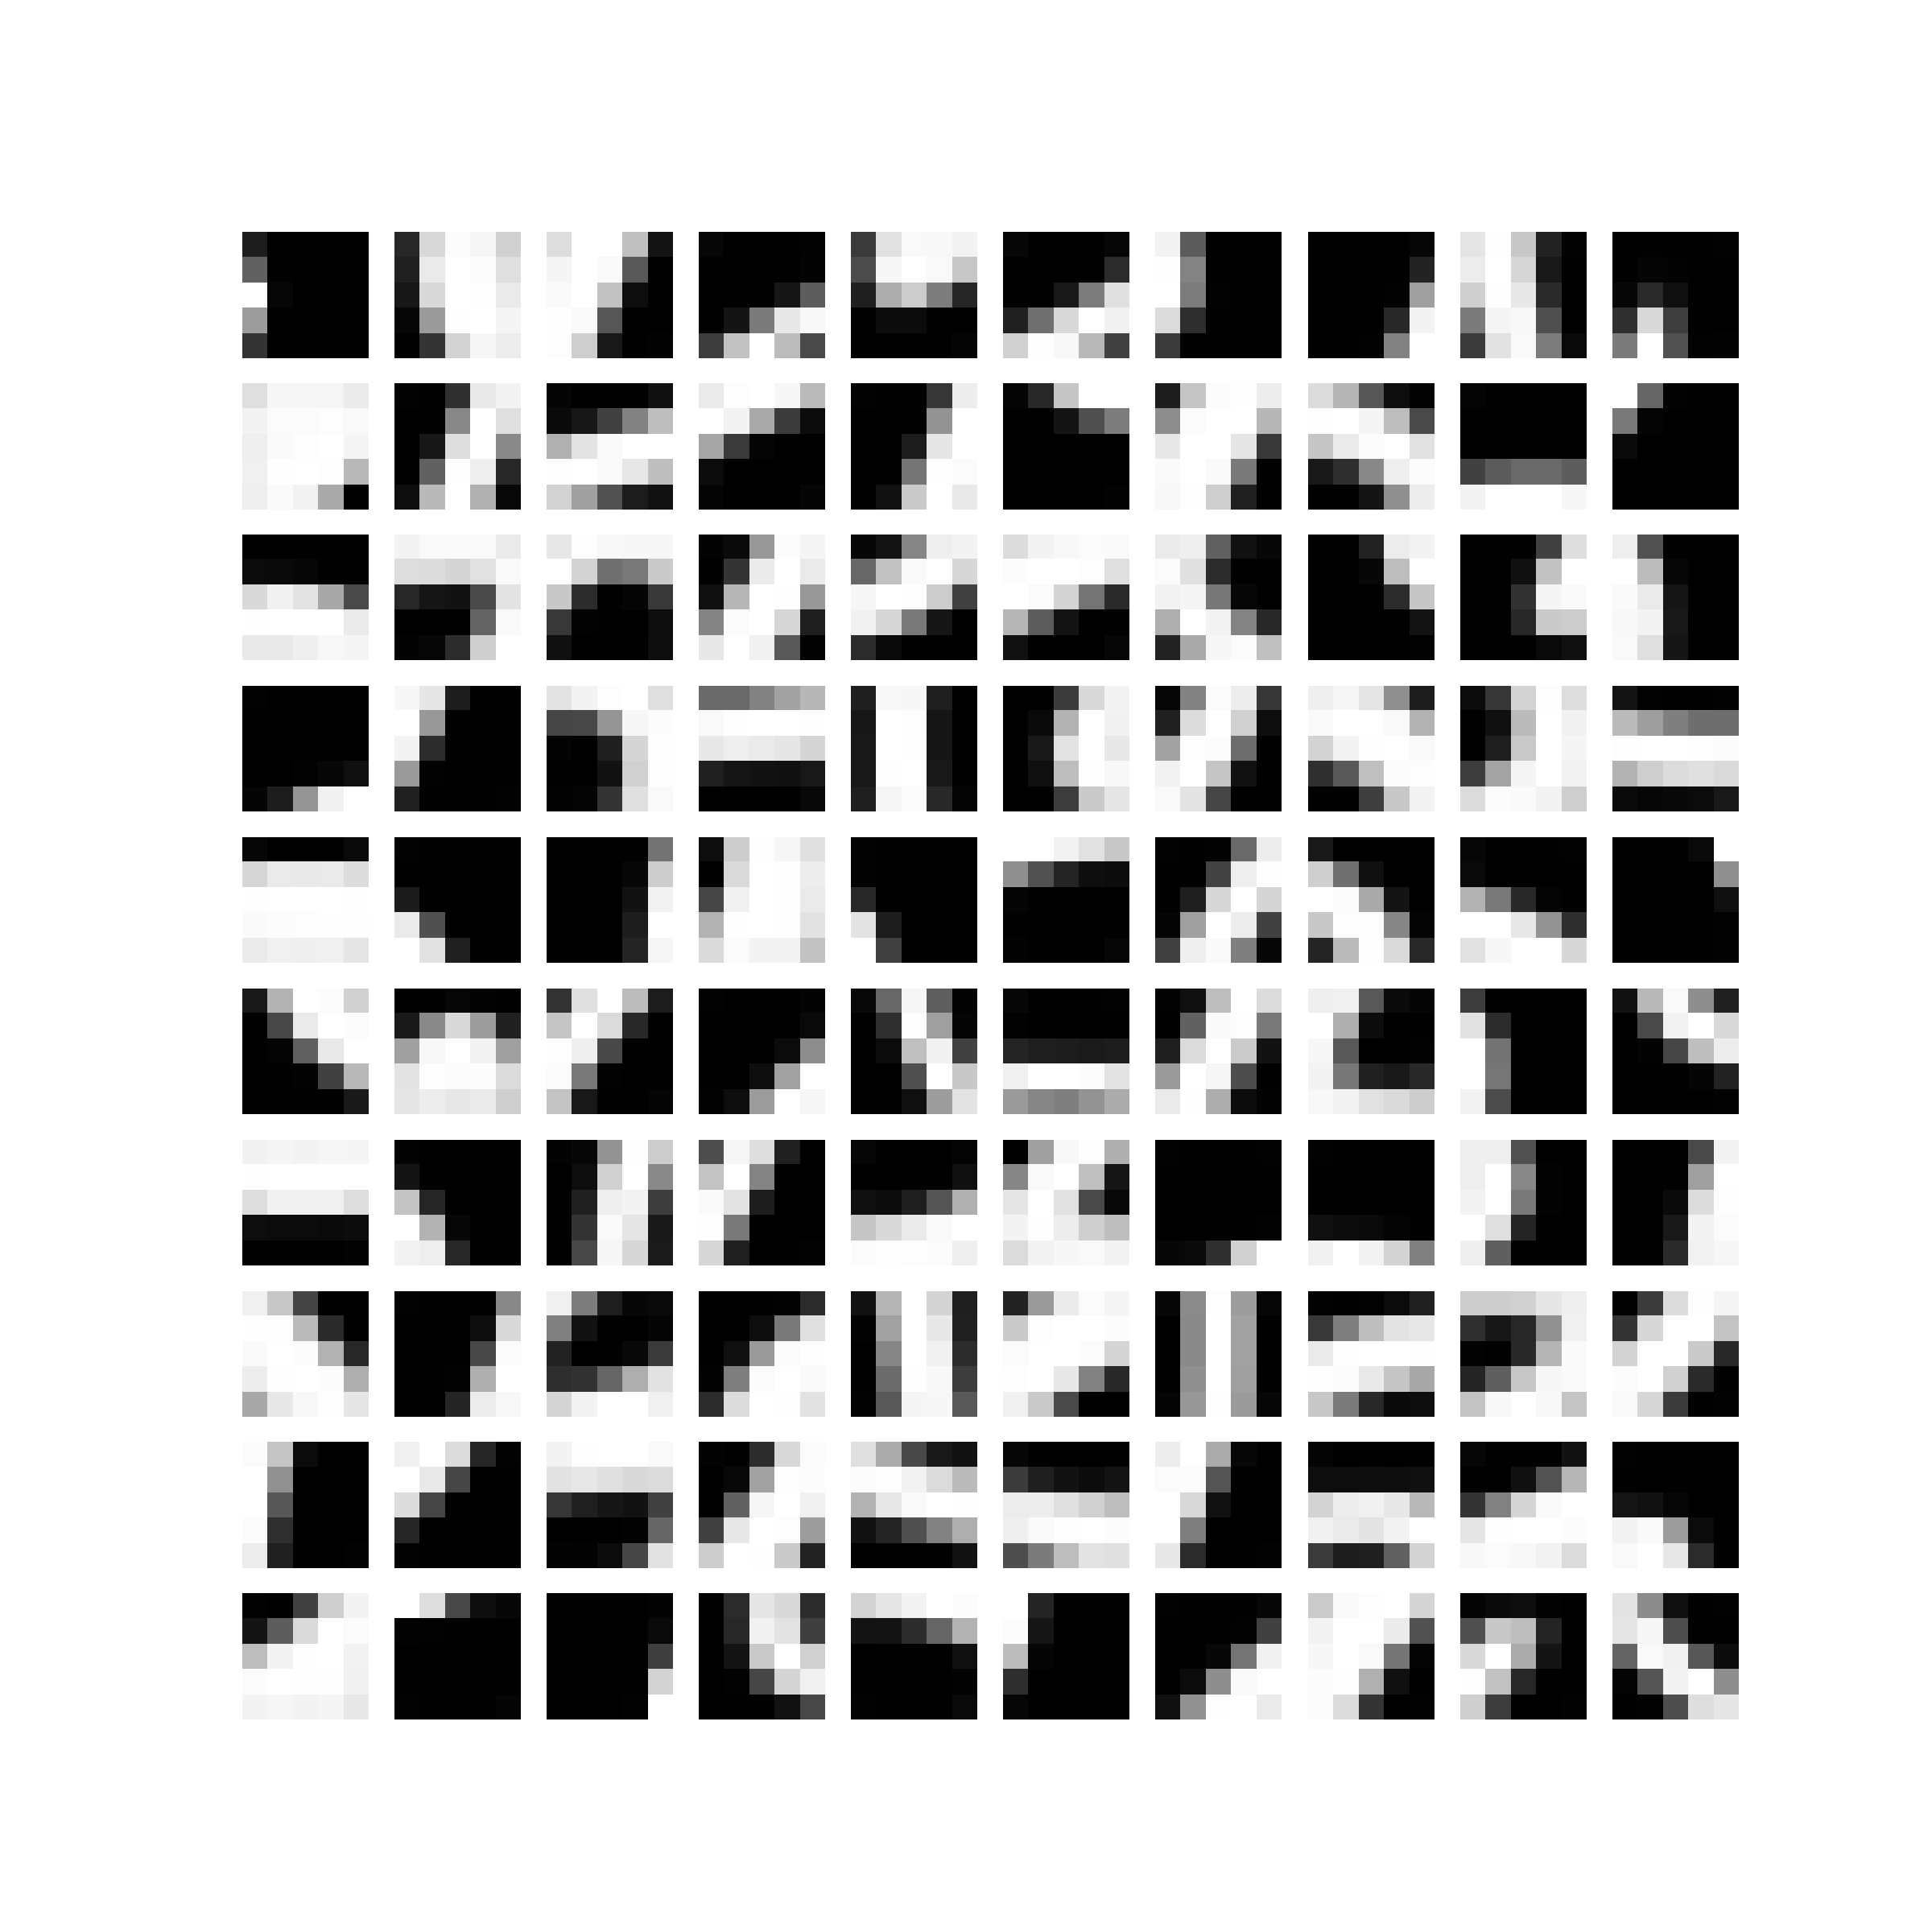
\includegraphics[width=\textwidth]{K-means/Result/Centroids/1000-clusters-centroids.png}
        \caption{ $K = 1000$}
        \label{fig:1000-centroids}
    \end{minipage}
\item $K = 5000, 10000$    
    % Third row
    \begin{minipage}{0.4\textwidth}
        \centering
        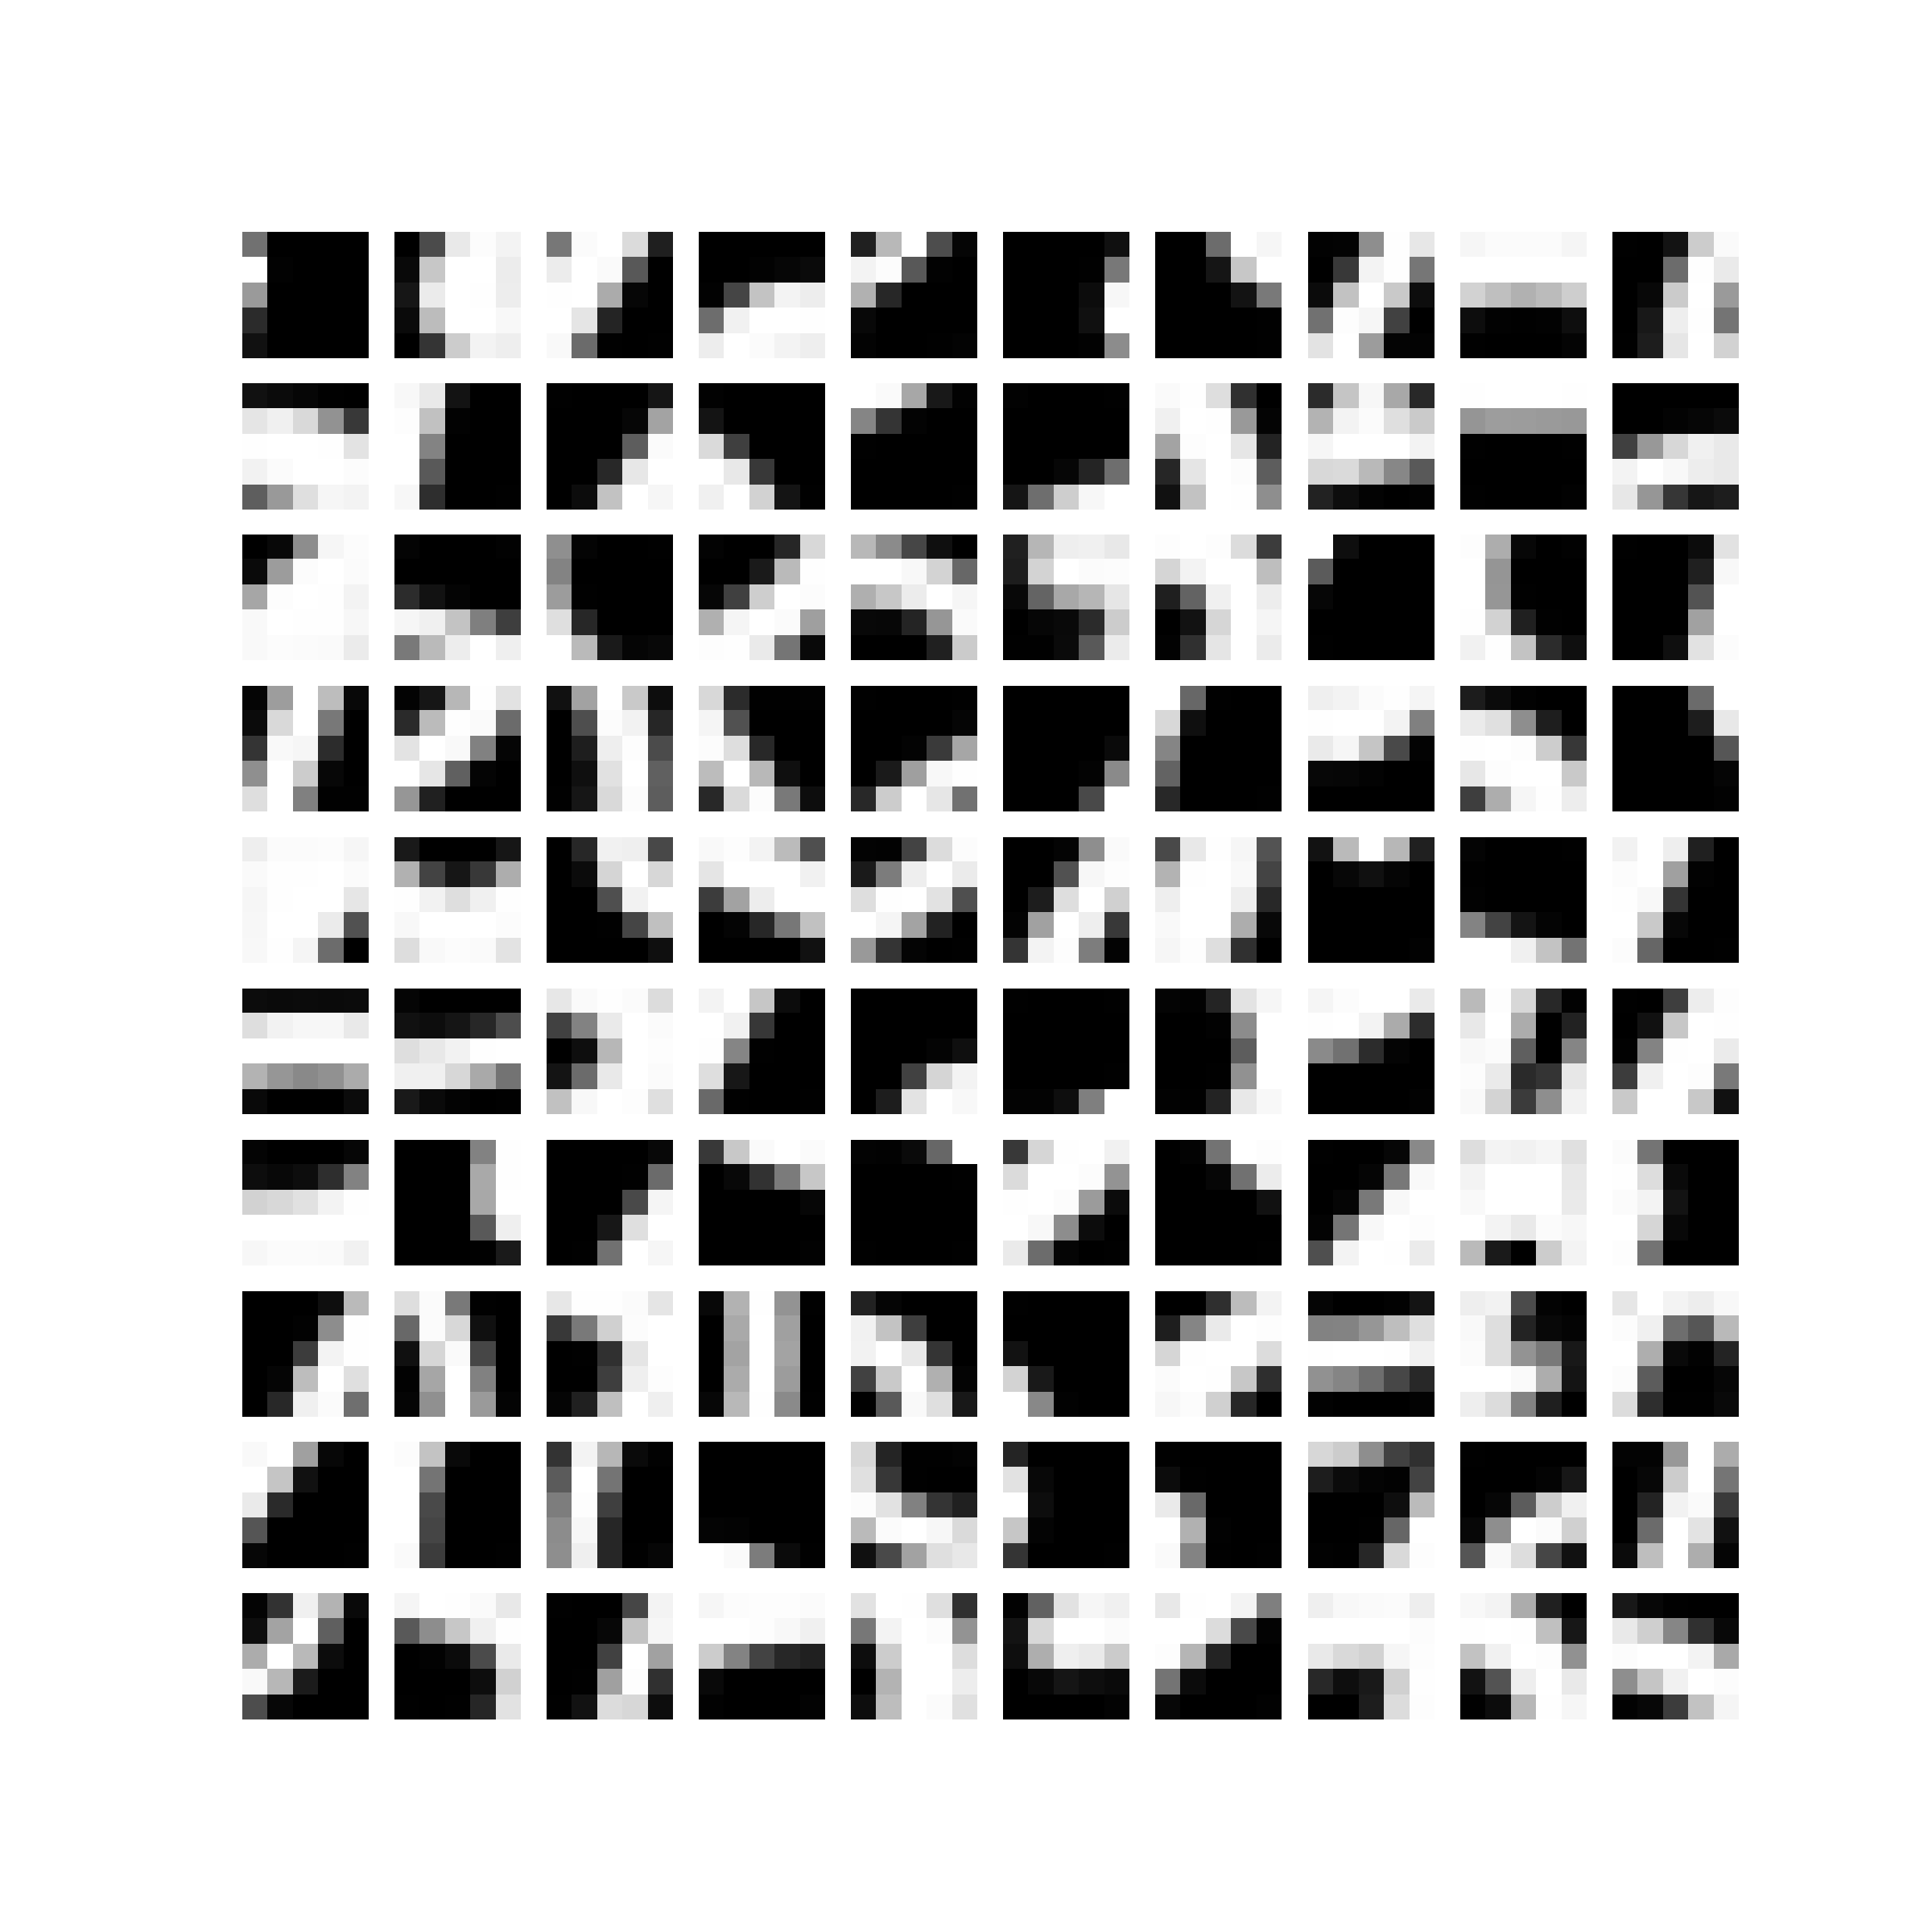
\includegraphics[width=\textwidth]{K-means/Result/Centroids/5000-clusters-centroids.png}
        \caption{$K = 5000$}
        \label{fig:5000-centroids}
    \end{minipage}%
    \begin{minipage}{0.4\textwidth}
        \centering
        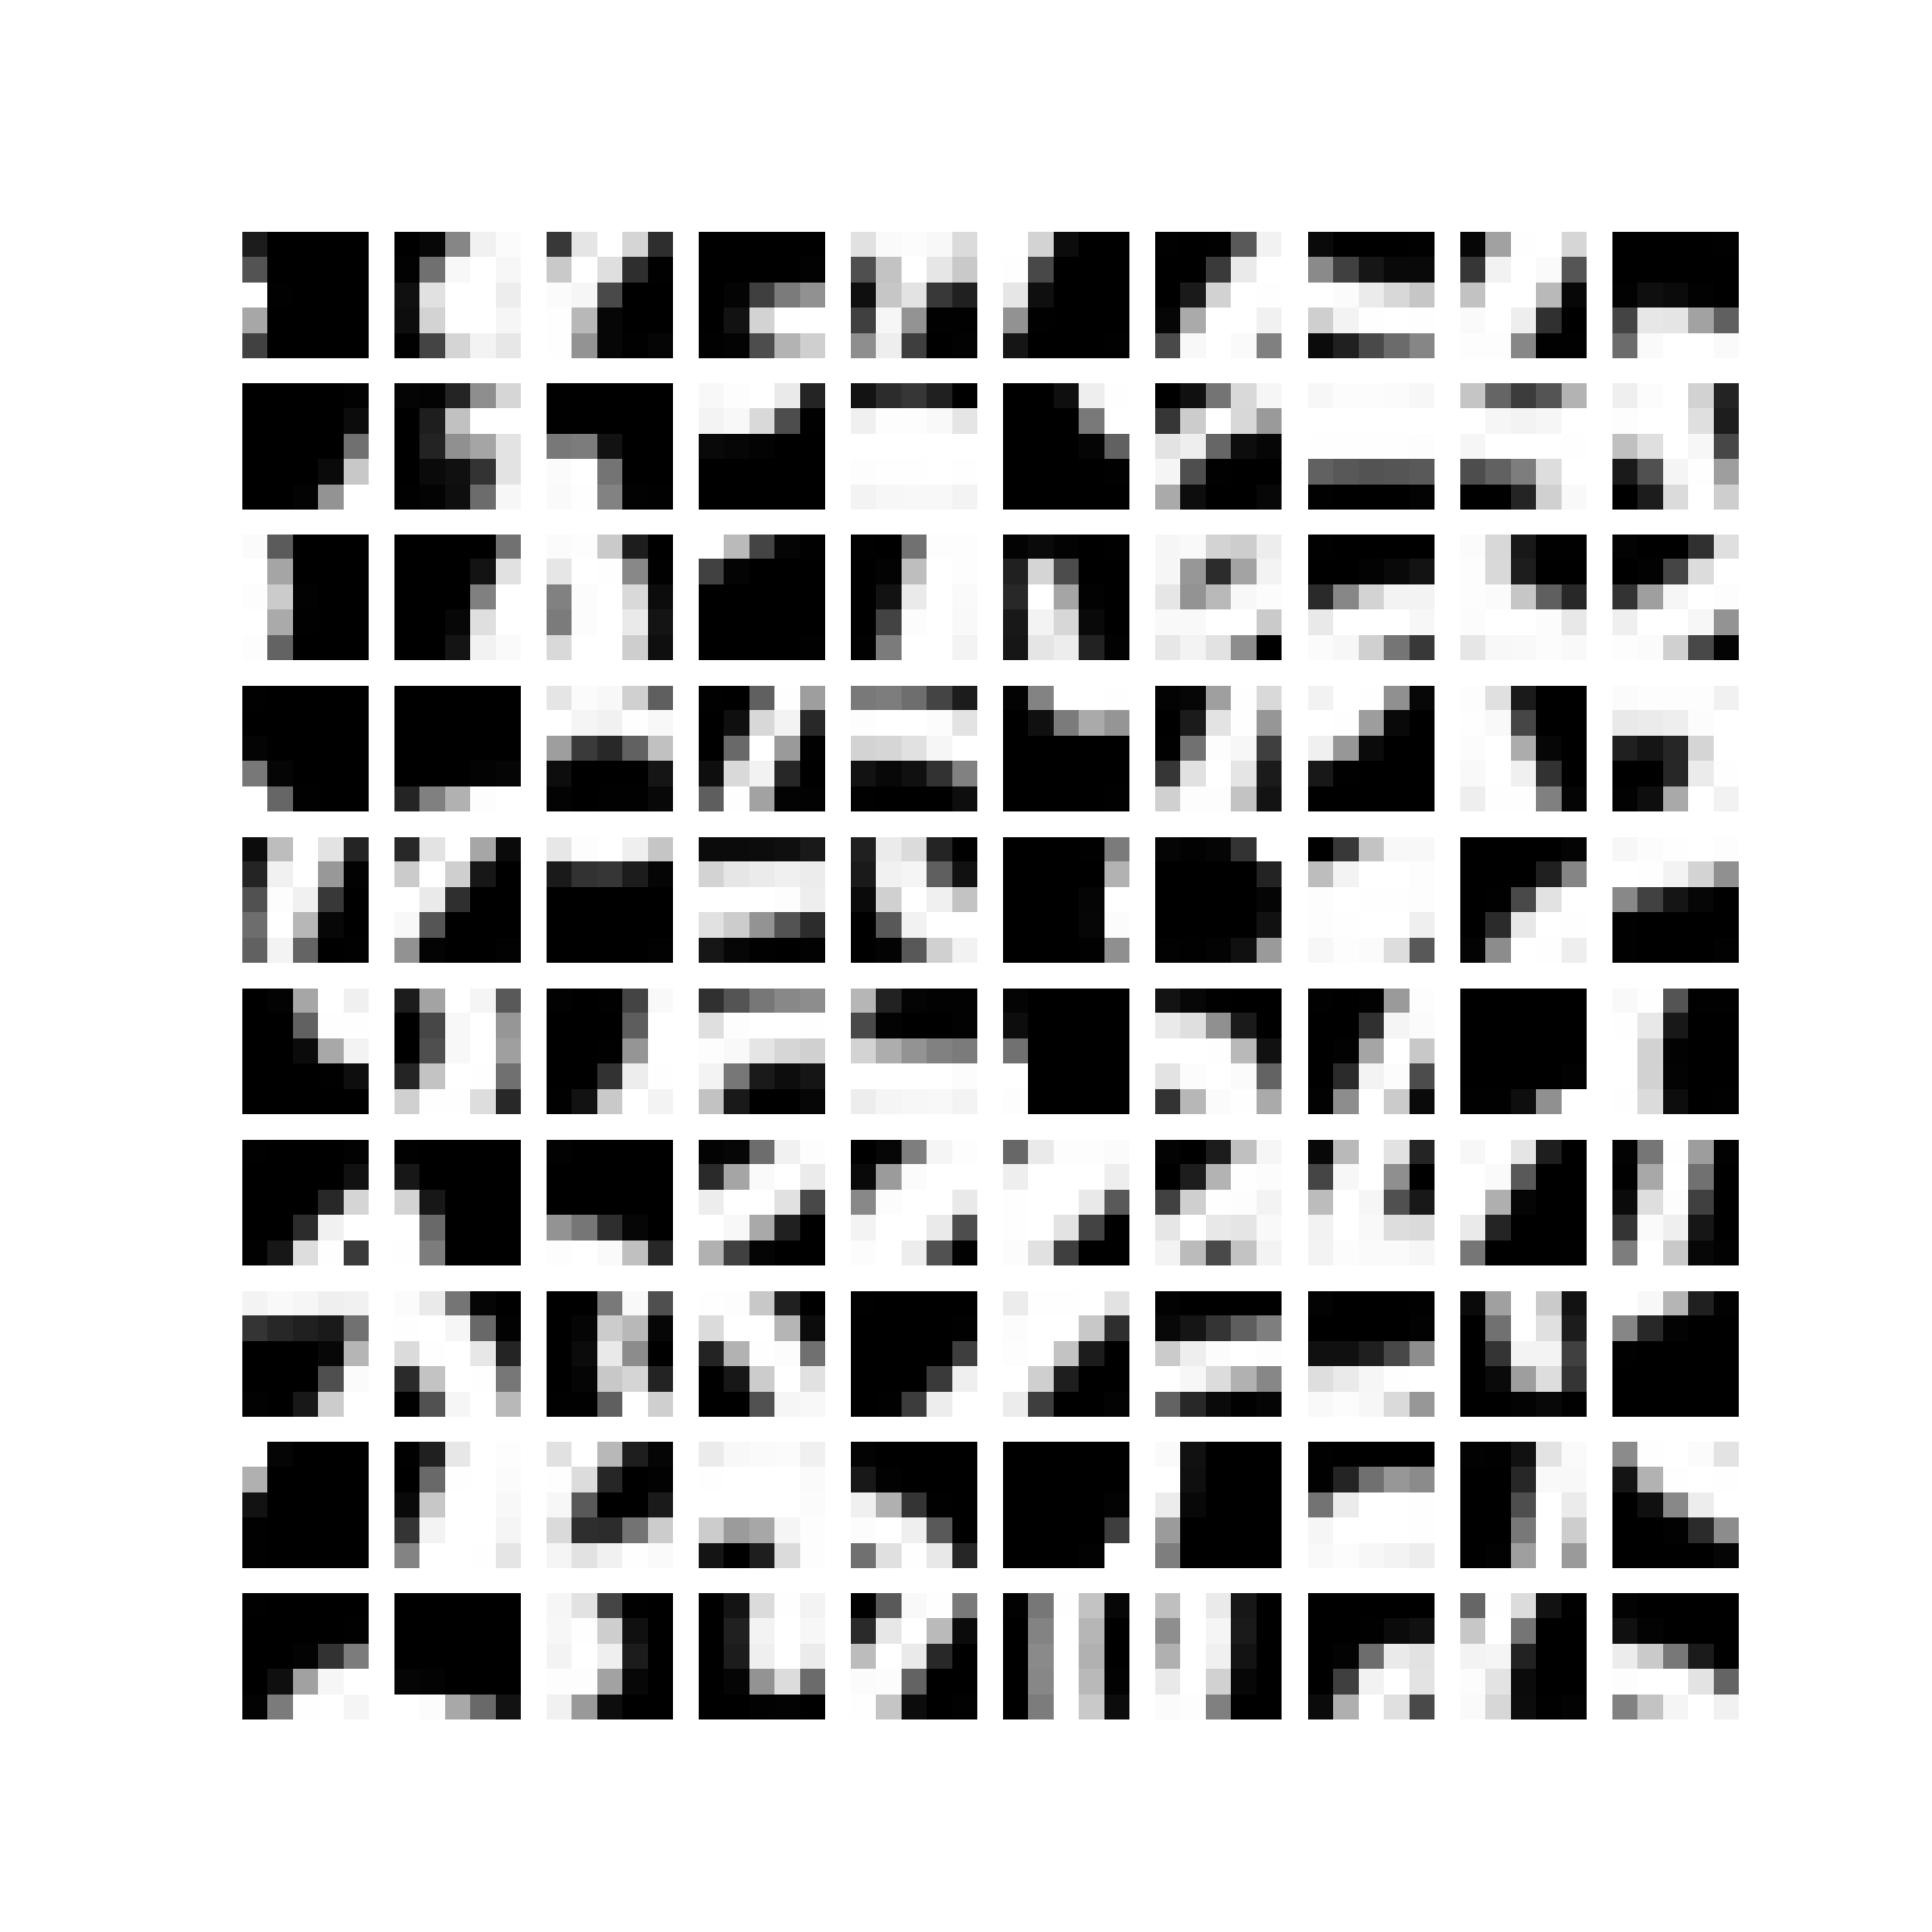
\includegraphics[width=\textwidth]{K-means/Result/Centroids/10000-clusters-centroids.png}
        \caption{$K = 10000$}
        \label{fig:10000-centroids}
    \end{minipage}
\end{figure}
    
\end{itemize}
\clearpage

\subsection{Reconstruction Performance}

As the algorithm illustrated in \textbf{2.2}, we do the reconstruction on the digit to test the performance of the K-mean clustering.

First, below is the example of the reconstruction result of the hand-written digit 2:

\begin{figure}[htbp!]
    \centering
    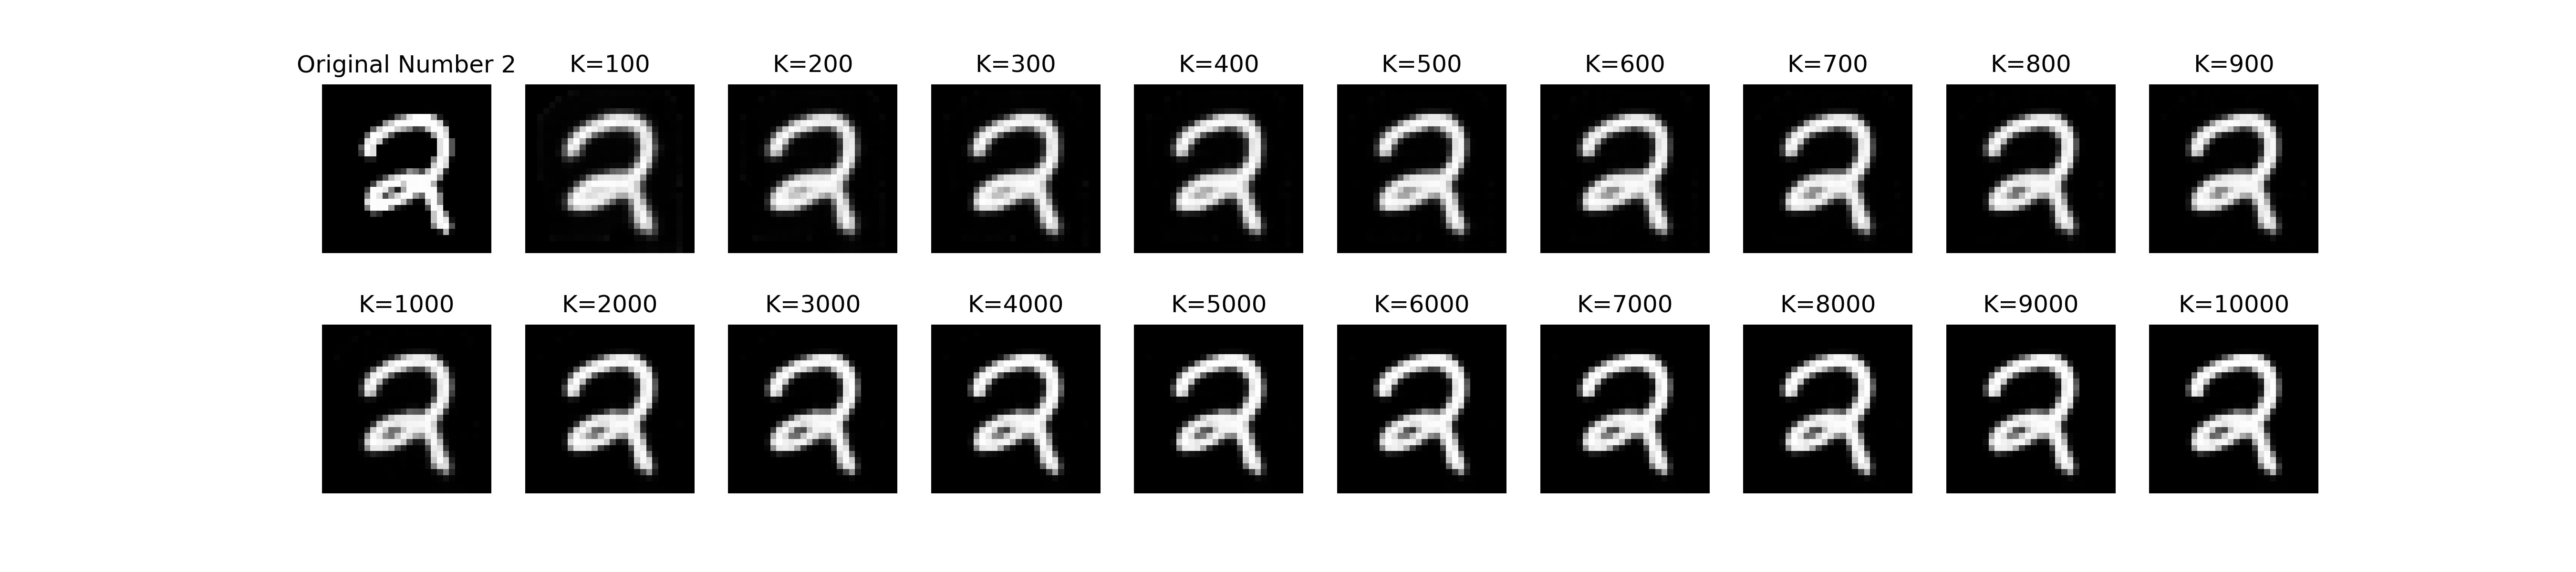
\includegraphics[width = \textwidth]{K-means/Result/Digits/reconstruct-digit.png}
    \caption{Reconstruction of digit 2 with different $K$}
    \label{fig:enter-label}
\end{figure}

We can see that:

\begin{itemize}
    \item when $K = 100$, it is okay for human beings to observe that the digit is a 2
    \item ???
\end{itemize}


Below is the overall MSE error of the reconstruction, and it should be noted that no normalization is used here. 

The Mean Squared Error (MSE) between two matrices \( D \) and \( \hat{D} \), each of size \( 28 \times 28 \), is given by:
\[
MSE = \frac{1}{28^2} \sum_{i=1}^{28} \sum_{j=1}^{28} (D_{ij} - \hat{D}_{ij})^2
\]
where \( D_{ij} \) and \( \hat{D}_{ij} \) are the elements at the \( i \)-th row and \( j \)-th column of matrices \( D \) and \( \hat{D} \), respectively.

\begin{figure}[htbp!]
    \centering
    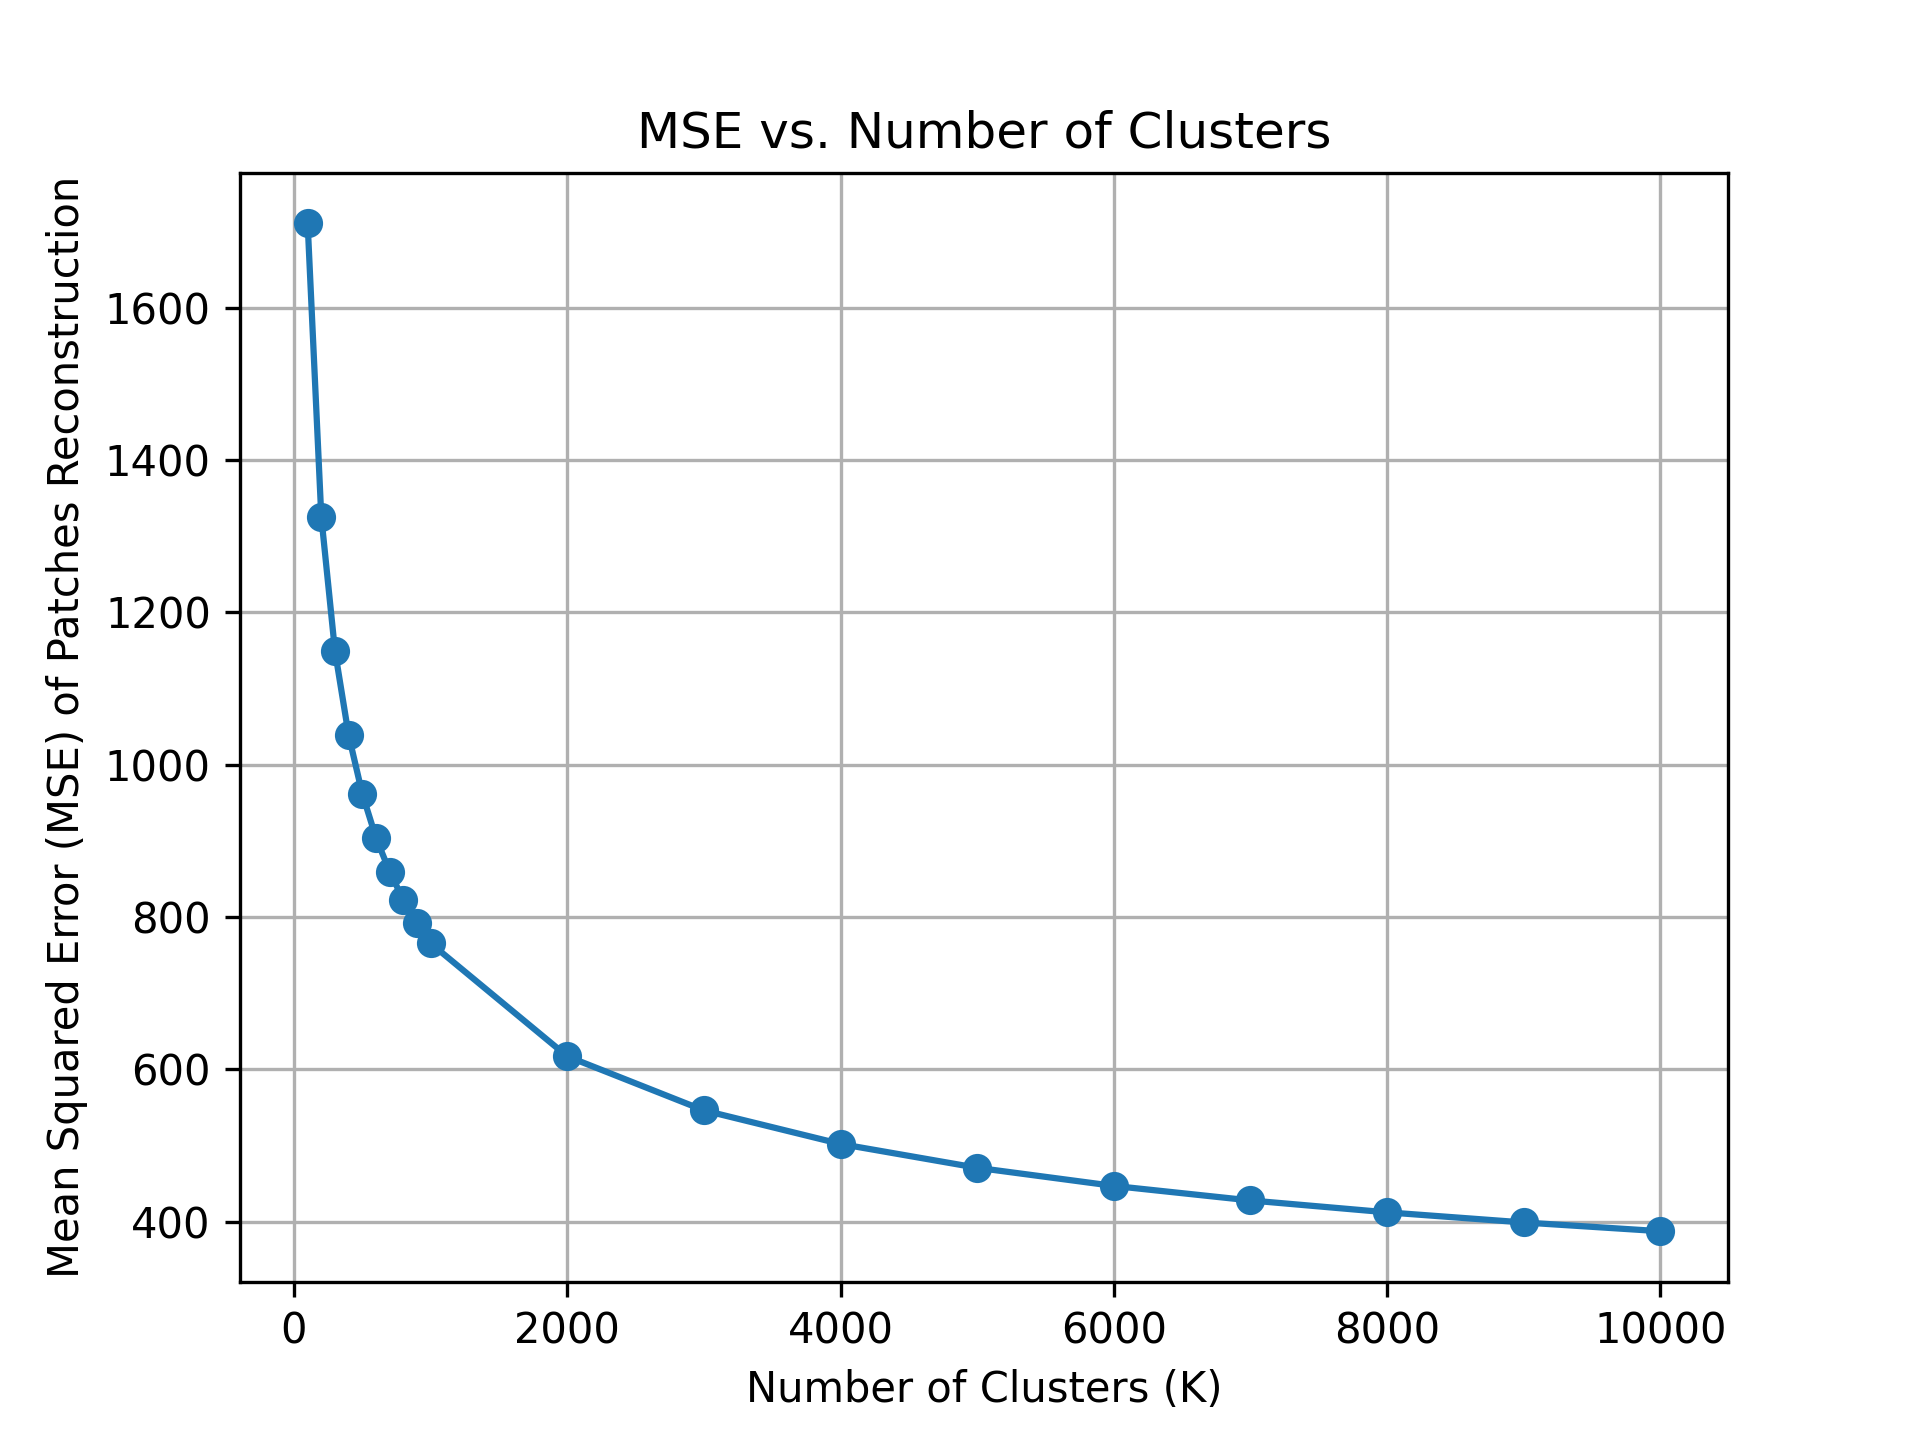
\includegraphics[width = 0.6 \textwidth]{K-means/Result/Patches/MSE_vs_K.png}
    \caption{MSE with different clustering number}
    \label{fig:enter-label}
\end{figure}
\section{Conclusion}


\printbibliography
\end{document}
